En este capítulo se analizan los resultados de la metodología propuesta al fenómeno de robo de vehículos. En la sección \ref{sec:data} se describe la fuente de información utilizada. En la sección \ref{sec:data_processing} los resultados del procesamiento de los datos. Por último, en la sección \ref{sec:quantative}-\ref{sec:qualitative} se realiza un análisis cuantitativo y cualitativo de los resultados.

\section{Datos}
\label{sec:data}

Para este experimento se cuenta con relatos de víctimas del robo de vehículos provistos por la Asociación de Aseguradores de Chile (AACH). Esta base de datos consta con 49,015 relatos entre los años 2011-2016, veasé la Figura \ref{img:robberies_aach} para el detalle por año.

\begin{figure}
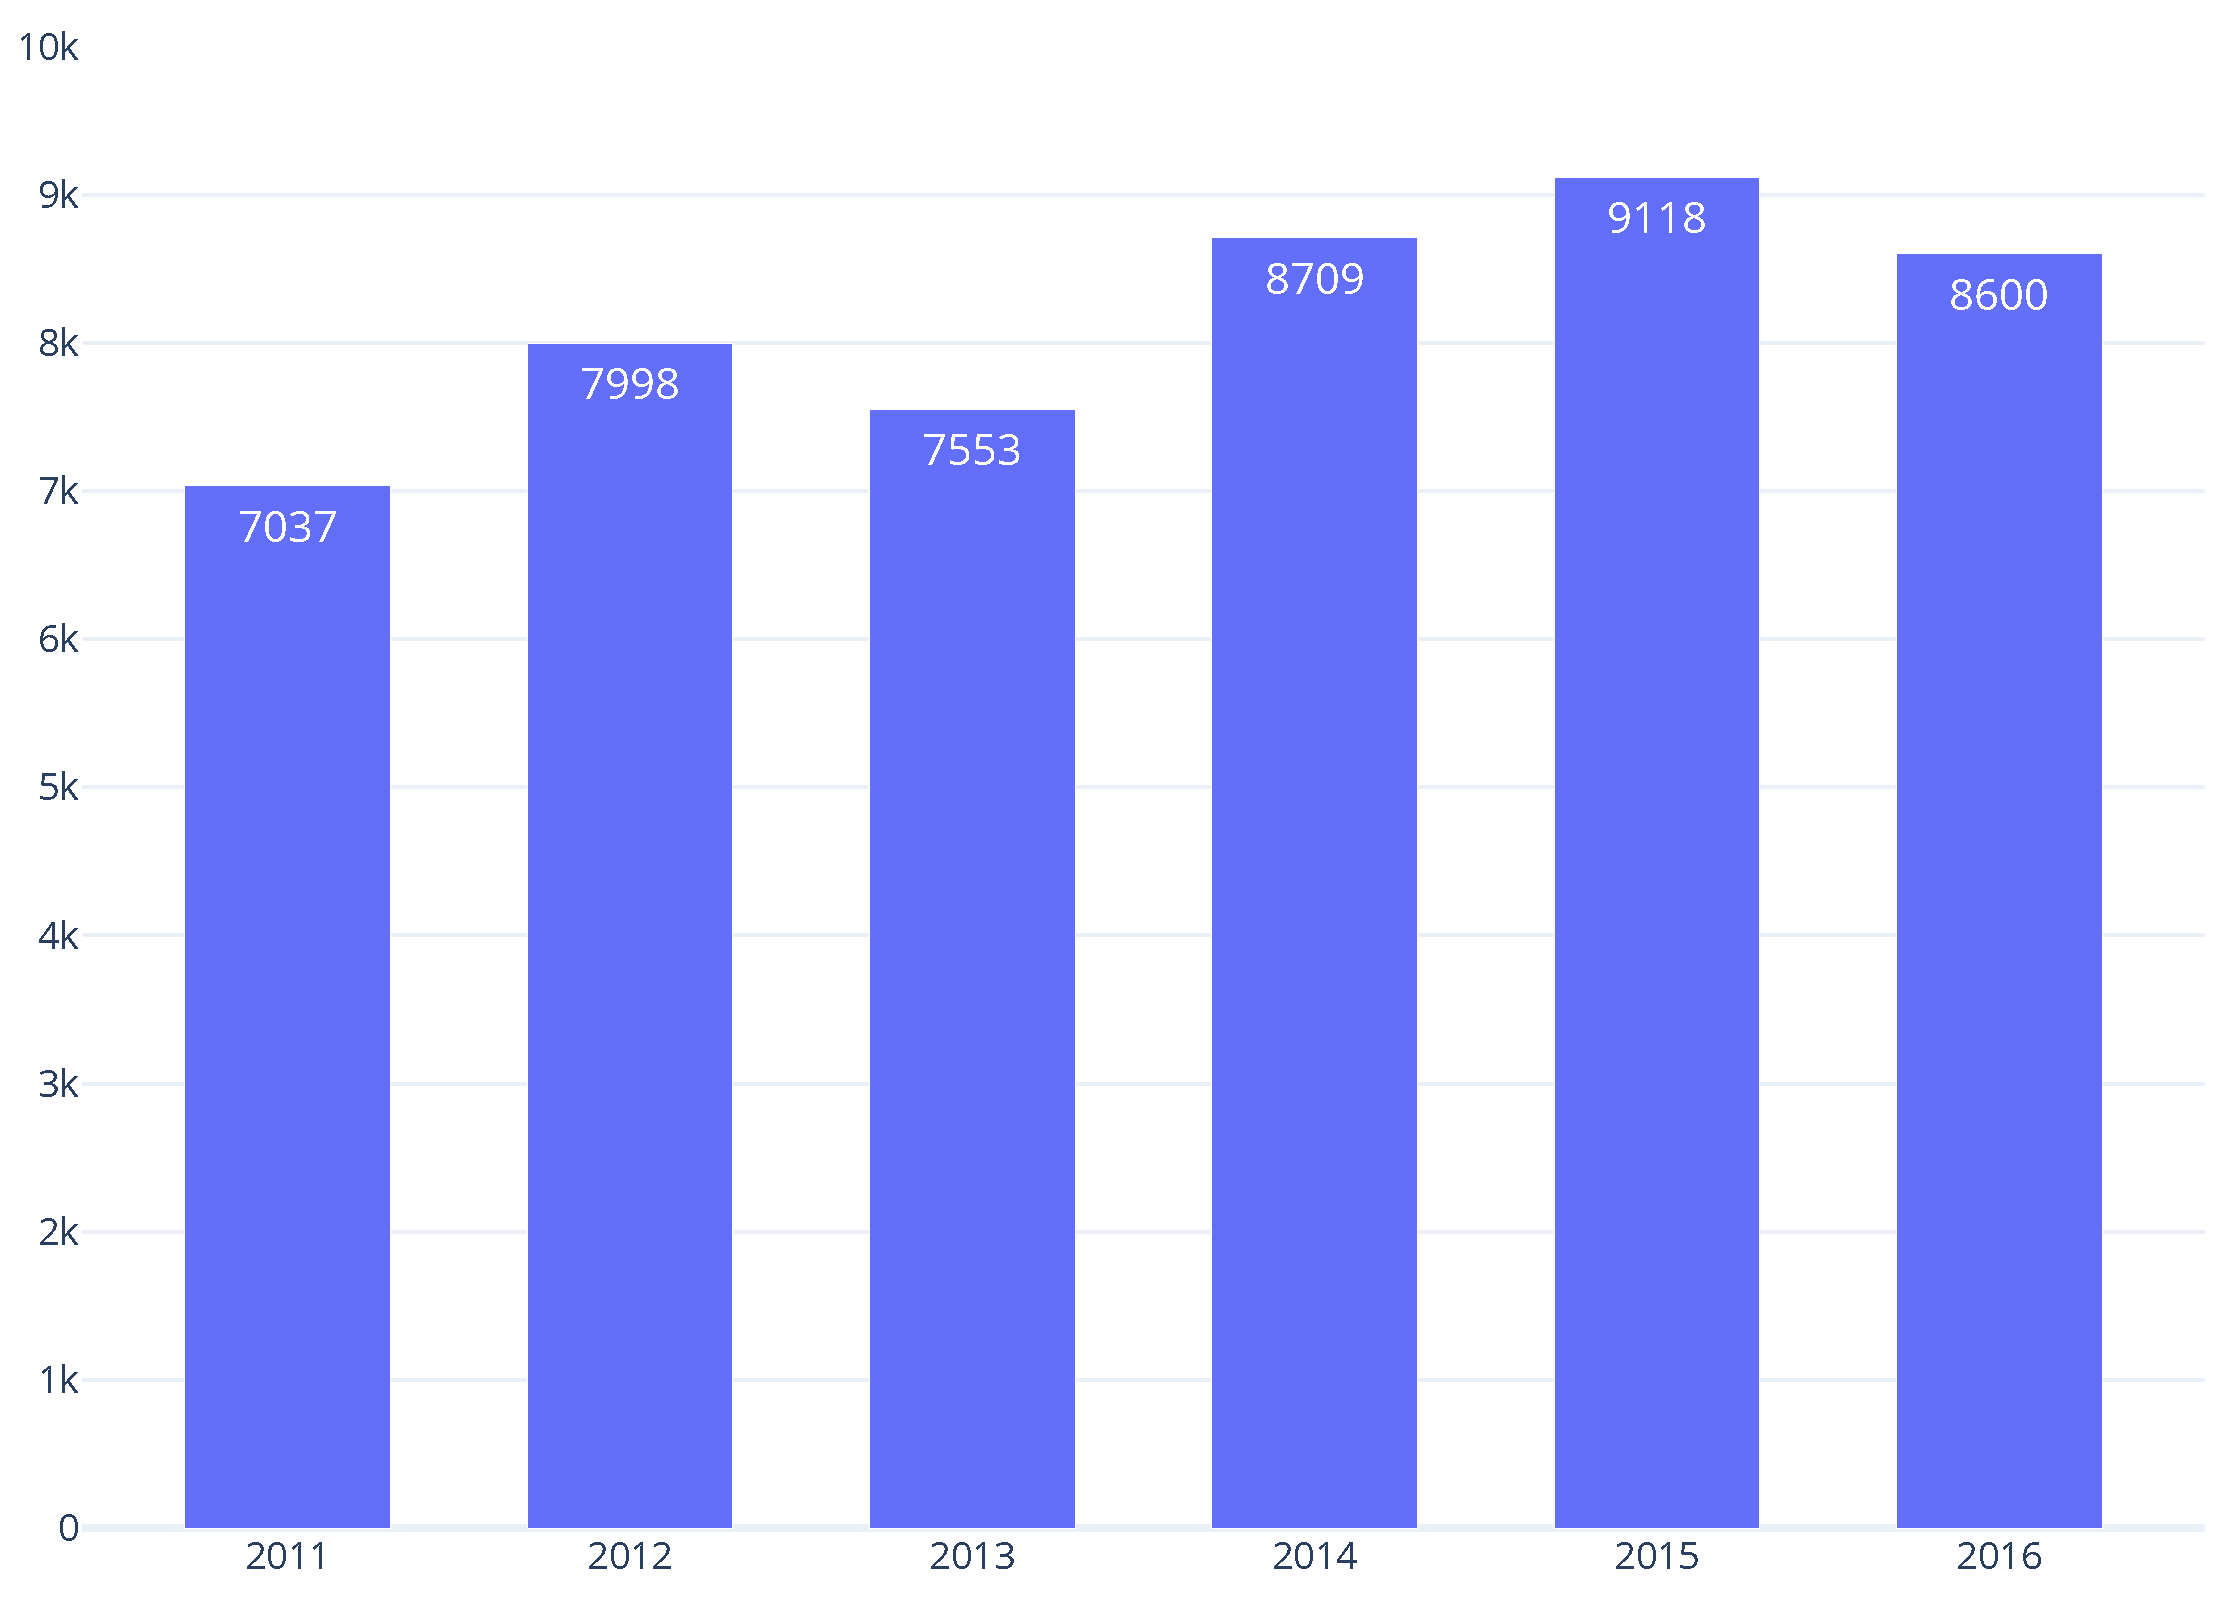
\includegraphics[width=0.8\textwidth]{ch4/robberies_aach.eps}
\caption{Cantidad de robos registrados por año en base de datos AACH.}
\label{img:robberies_aach}
\end{figure}

En la Figura \ref{img:documents} se muestra algunos ejemplos de la base de datos de la AACH, de aquí se observa que los relatos carecen de estandarización y presentan múltiples errores ortográficos. En consecuencia, la etapa de procesamiento toma suma relevancia, ya que aplicar un modelo de tópicos a un corpus sin ningún tipo de procesamiento puede llevar a resultados no deseados. En la sección \ref{sec:data_processing} se detallan los resultados obtenidos sobre el corpus tras aplicar los niveles de procesamiento mencionados en la sección \ref{sec:processing}.

\def\grayboxtext[#1,#2]#3{
        \node[fill=gray!80, text width=36em, draw=black!80, rounded corners, align=justify, below=#1] (#2) {#3}; 
}
\begin{figure}
\begin{tikzpicture}
    \grayboxtext[,t1]{\small ESTABA ESTACIONADO EL LA CALLE ROTEMBURGO ENTRE NORUGA Y SEÑORA DEL ROSAIO  Y AL MOMENTO DE IR A BUSCAR EL AUTO SE DA CUENTA QUE EL VH NO SE ENCUETRA AL PARECER LO ROBARON. NO POSEEE LOS DOCUMENTOS DEL VH vh aparece pero con mulples daños e evaluar queda en manos del liquidador.};
    \grayboxtext[0.2cm of t1,t2]{\small ME ENCONTRABA CARGANDO COMBUSTIBLE EN LA SHELL DE CARRASCAL CON WALKER MARTÍNEZ Y REPENTINAMENTE FUI ASALTADA EN FORMA VIOLENTA LLEVASE MI VEH (TENGO GRABACIÓN ). DAÑOS: ROBO DE MI VEH . LEIVA SE DERIVA A DON MARIO MEDINA .3 UF.DED/XX@XX.CL};
    \grayboxtext[0.2cm of t2,t3]{\small TEXT : DEJO MI VEHICULO ESTACIONADO EN DICHO LUGAR AL VOLVER ME PERCATO QUE EL VEHICULO HABIA SIDO ROBADO  EL MISMO DIA DEL ROBO A LAS 20:00 SOY CONTACTADO POR CARABINEROS DE LA COMUNA DE EL BOSQUE LOS CUALES ME INFORMAN QUE HABIAN RECUPERADO MI VEHICULO EL CUAL PRESENTABA LOS SIGUIENTES DAÑOS : VIDRIO TRASERO DERECHO QUEBRADA  CHAPA DE CONTACTO FORZADA  PARACHOQUE DELANTERO DERECHO RAYADO  ALARMADESCONECTADA  OTROS DAÑOS EN EL SISTEMA ELECTRICO  ALARMA DE AIRBAGS ENCENDIDA  ROBO DE ESPECIES.};
    \grayboxtext[0.2cm of t3,t4]{\small Descripción Siniestro: el dia 24 de abril se le arrendo el vh a XX el cual estuvo sin problemas pagando el arriendo  hasta el mes pasado que no pago mas y se le ha llamado en reiteradas veces y dice que va a venir a dejar el auto y no aparecel. por eso se realizo una denuncia por apropiacion indevida};
    \grayboxtext[0.2cm of t4,t5]{\small ammg  53966748    vh asegurado transitaba en calle copiapo alt. 750  en este punto sufro portonazo sujetos armados roban mi vh hoy a las 04.30am vh fue encontrado en sector de la pintana mi vh ahora esta siendo periciado.    daños por evaluar};
    \grayboxtext[0.2cm of t5,t6]{\small PATENTE XX Siendo las 22:30 en la interseccion de san Alfonso con Claudio Gay  un individuo me obliga a bajar del vehiculo apuntandome con una pistola  de inmediato aparecen dos personas mas  las que me suben en la parte trasera del furgon donde constantemente me amenazan con dispararme  me bajan del vehiculo en un potrero cercano a la autopista del sol  teniendome boca abajo golpeandome  luego me colocan un pa?o en la cara perdiendo el conocimiento  al despertar desorientado me dirijo a car};
\end{tikzpicture}
\caption{Muestra de relatos de la base de datos AACH.}
\label{img:documents}
\end{figure}

\section{Procesamiento}
\label{sec:data_processing}

En esta sección se detallan los resultados de aplicar el procesamiento descrito en la sección \ref{sec:processing}. Con fines gráficos los resultados del procesamiento se decriben en un orden distinto al descrito en dicha sección, con el objetivo de mostrar como estas afectan el tamaño del vocabulario. El orden es el siguiente, (i) tokenización, (ii) procesamiento de caracteres, (iii) eliminación de palabras poco frecuentes, (iv) filtro por vocabulario, (v) eliminación de \textit{stopwords} y (vi) eliminación de documentos con pocas palabras.\\

En primer lugar, se muestran la distribución acumulada del corpus original tras solo aplicar tokenización. Como se observa en la Figura \ref{img:cum_dist1} los \textit{tokens} totales corresponden a 2,030,980 asociado a un vocabulario de 93,203 palabras.\\

\begin{figure}
    \centering
    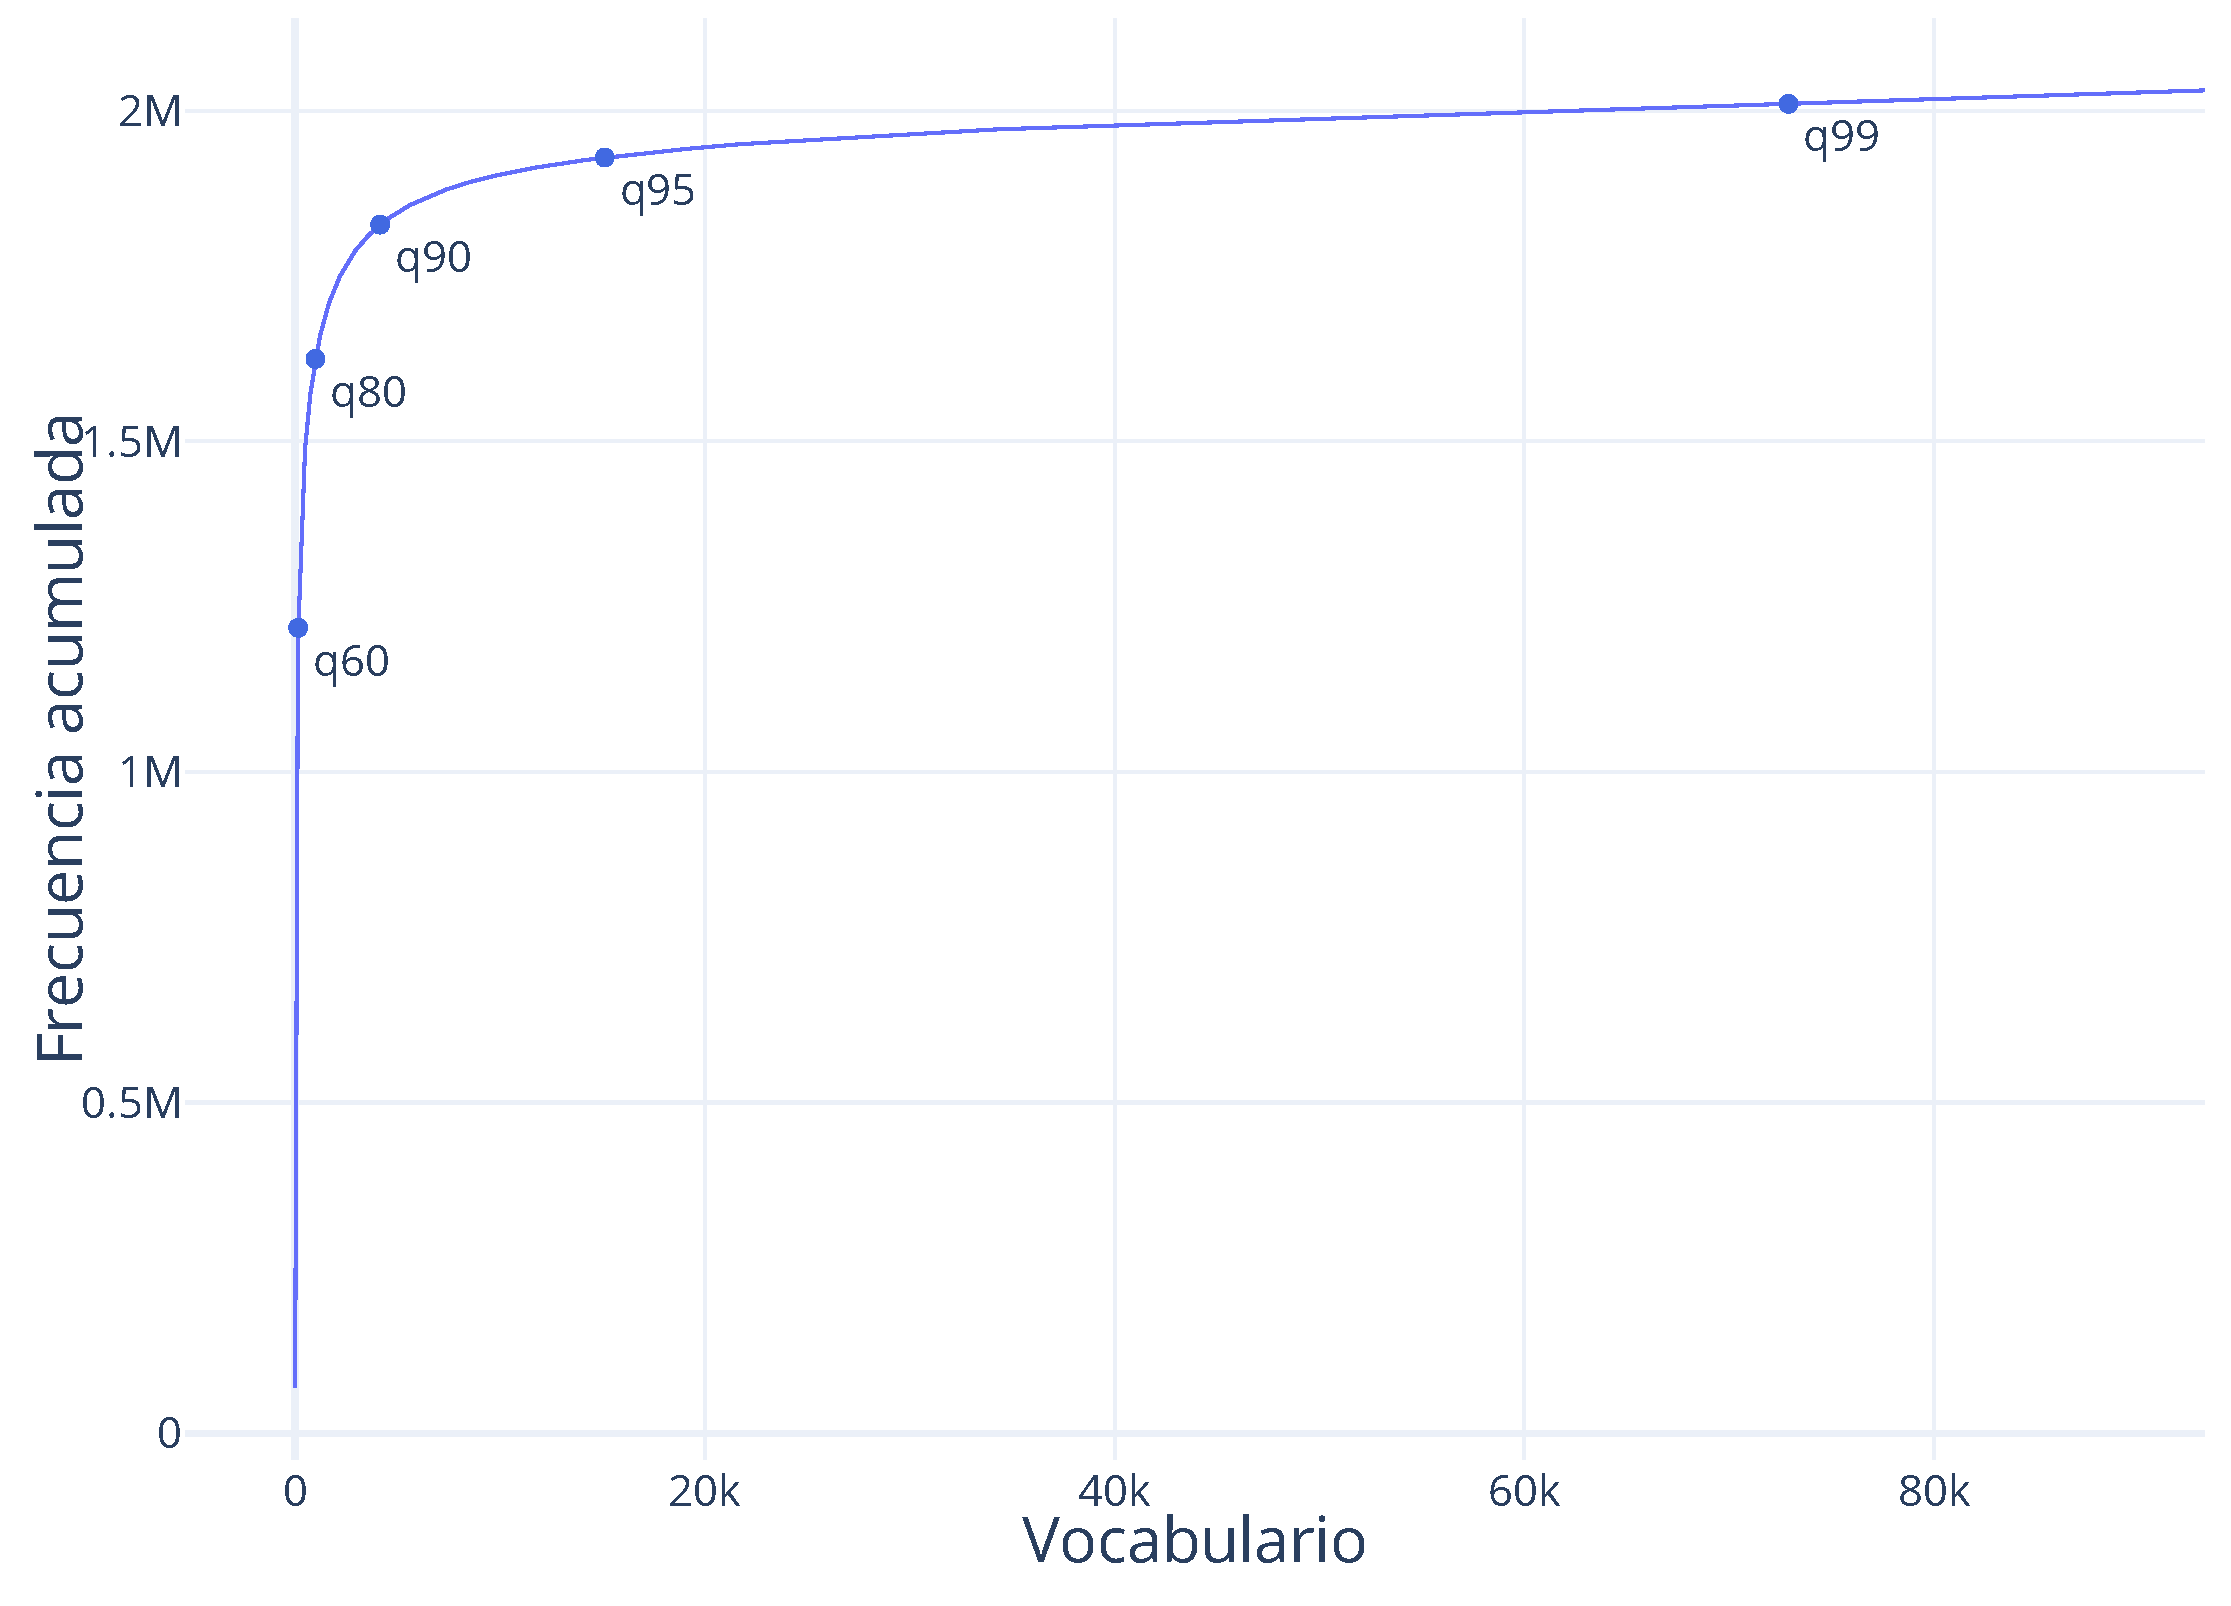
\includegraphics[trim={1.155cm 1.3cm 0 0},clip,width=0.6\textwidth]{ch4/cum_dist_1.eps}
    \caption{Frecuencia acumulada del vocabulario en orden decreciente de ocurrencia aplicando hasta el primer nivel de procesamiento.}
    \label{img:cum_dist1}
\end{figure}

En segundo lugar, se aplica la etapa de procesamiento de caracteres. De acuerdo a la Figura \ref{img:cum_dist2} el tamaño del vocabulario se reduce a casi la mitad, específicamente a 42,921 palabras, de forma similar la cantidad de \textit{tokens} se reduce a 1,028,412.

\begin{figure}
    \centering
    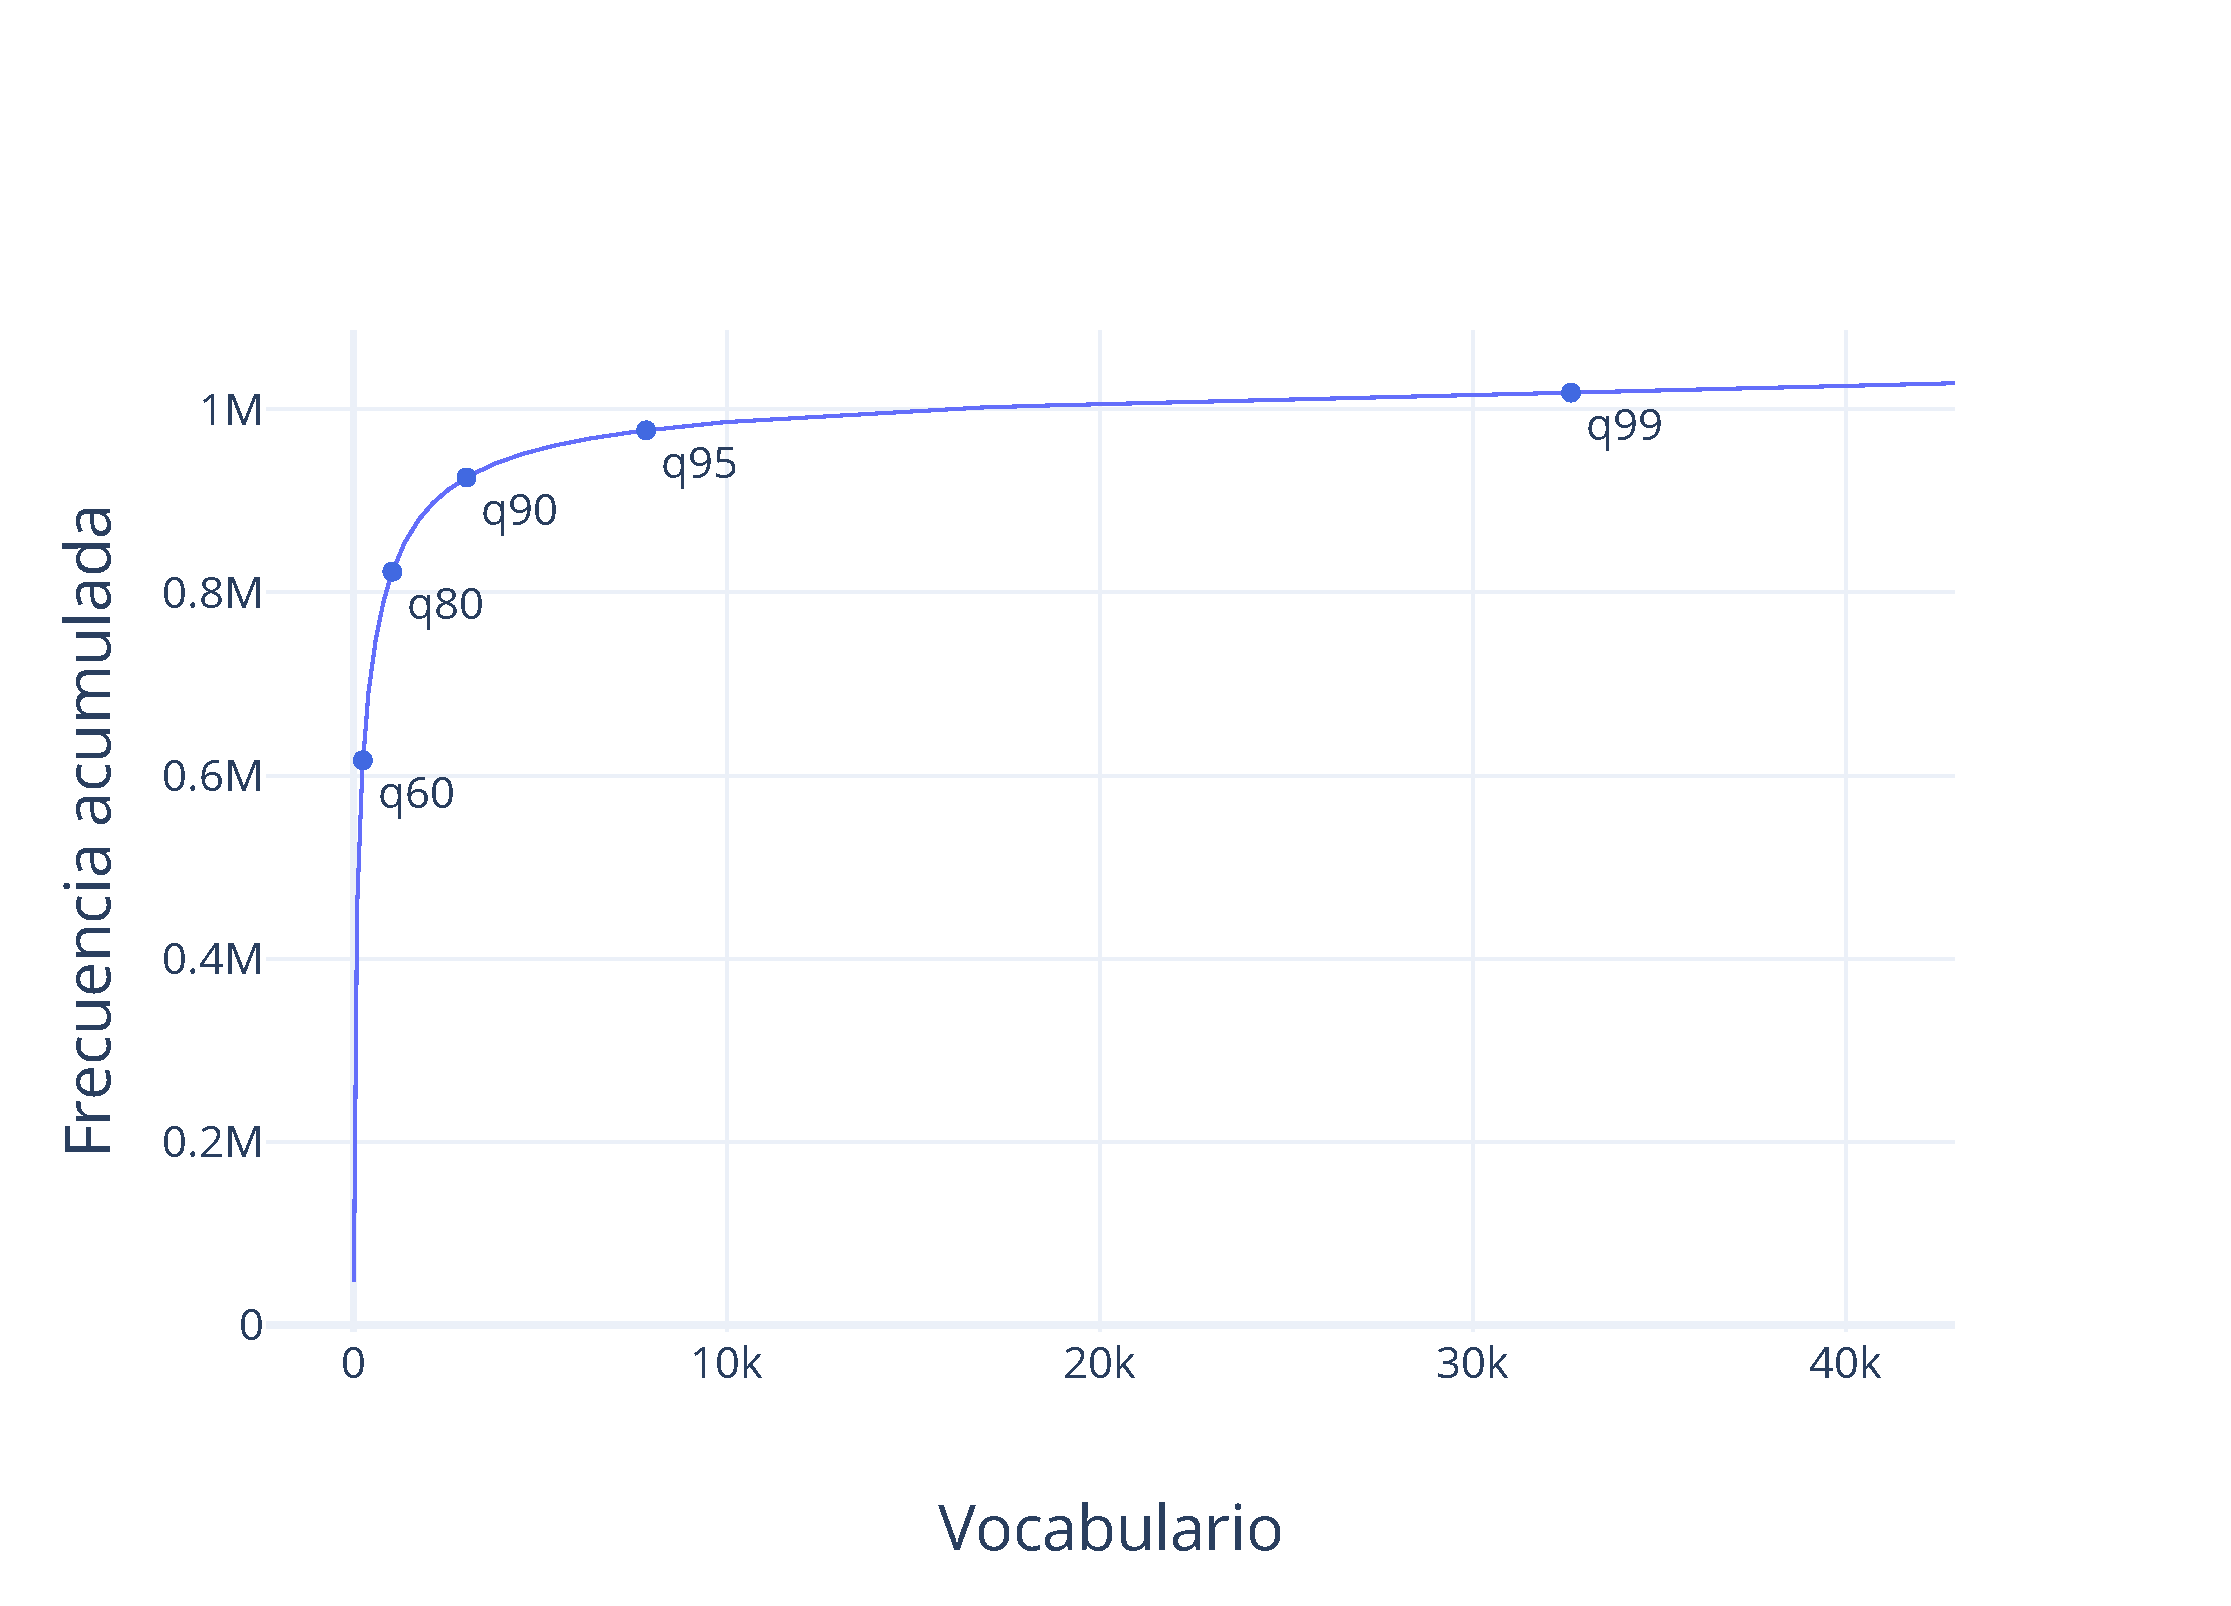
\includegraphics[trim={1.155cm 1.3cm 0 0},clip,width=0.6\textwidth]{ch4/cum_dist_2.eps}
    \caption{Frecuencia acumulada del vocabulario en orden decreciente de ocurrencia aplicando hasta el segundo nivel de procesamiento.}
    \label{img:cum_dist2}
\end{figure}

Hasta este nivel de procesamiento se tiene que cerca del 50\% de las palabras ocurren una única vez y al cerca de un 80\% tiene una frecuencia igual o menor a 4. El 95\% de la distribución acumulada puede ser explicada con 7,837 palabras (un 18\% del vocabulario actual). En conclusión, la distribución de las palabras tiene una cola bastante pesada.\\

En tercer lugar, se eliminan las palabras que aparecen en menos del 0.1\% de los documentos de su época. En la Figura \ref{img:cum_dist3} se muestra una reducción importante del vocabulario, específicamente a 3,148 (al rededor de 14 veces), reduciendo levemente  (alrededor de un 10\%) la cantidad de \textit{tokens} a 925,693.\\

\begin{figure}
    \centering
    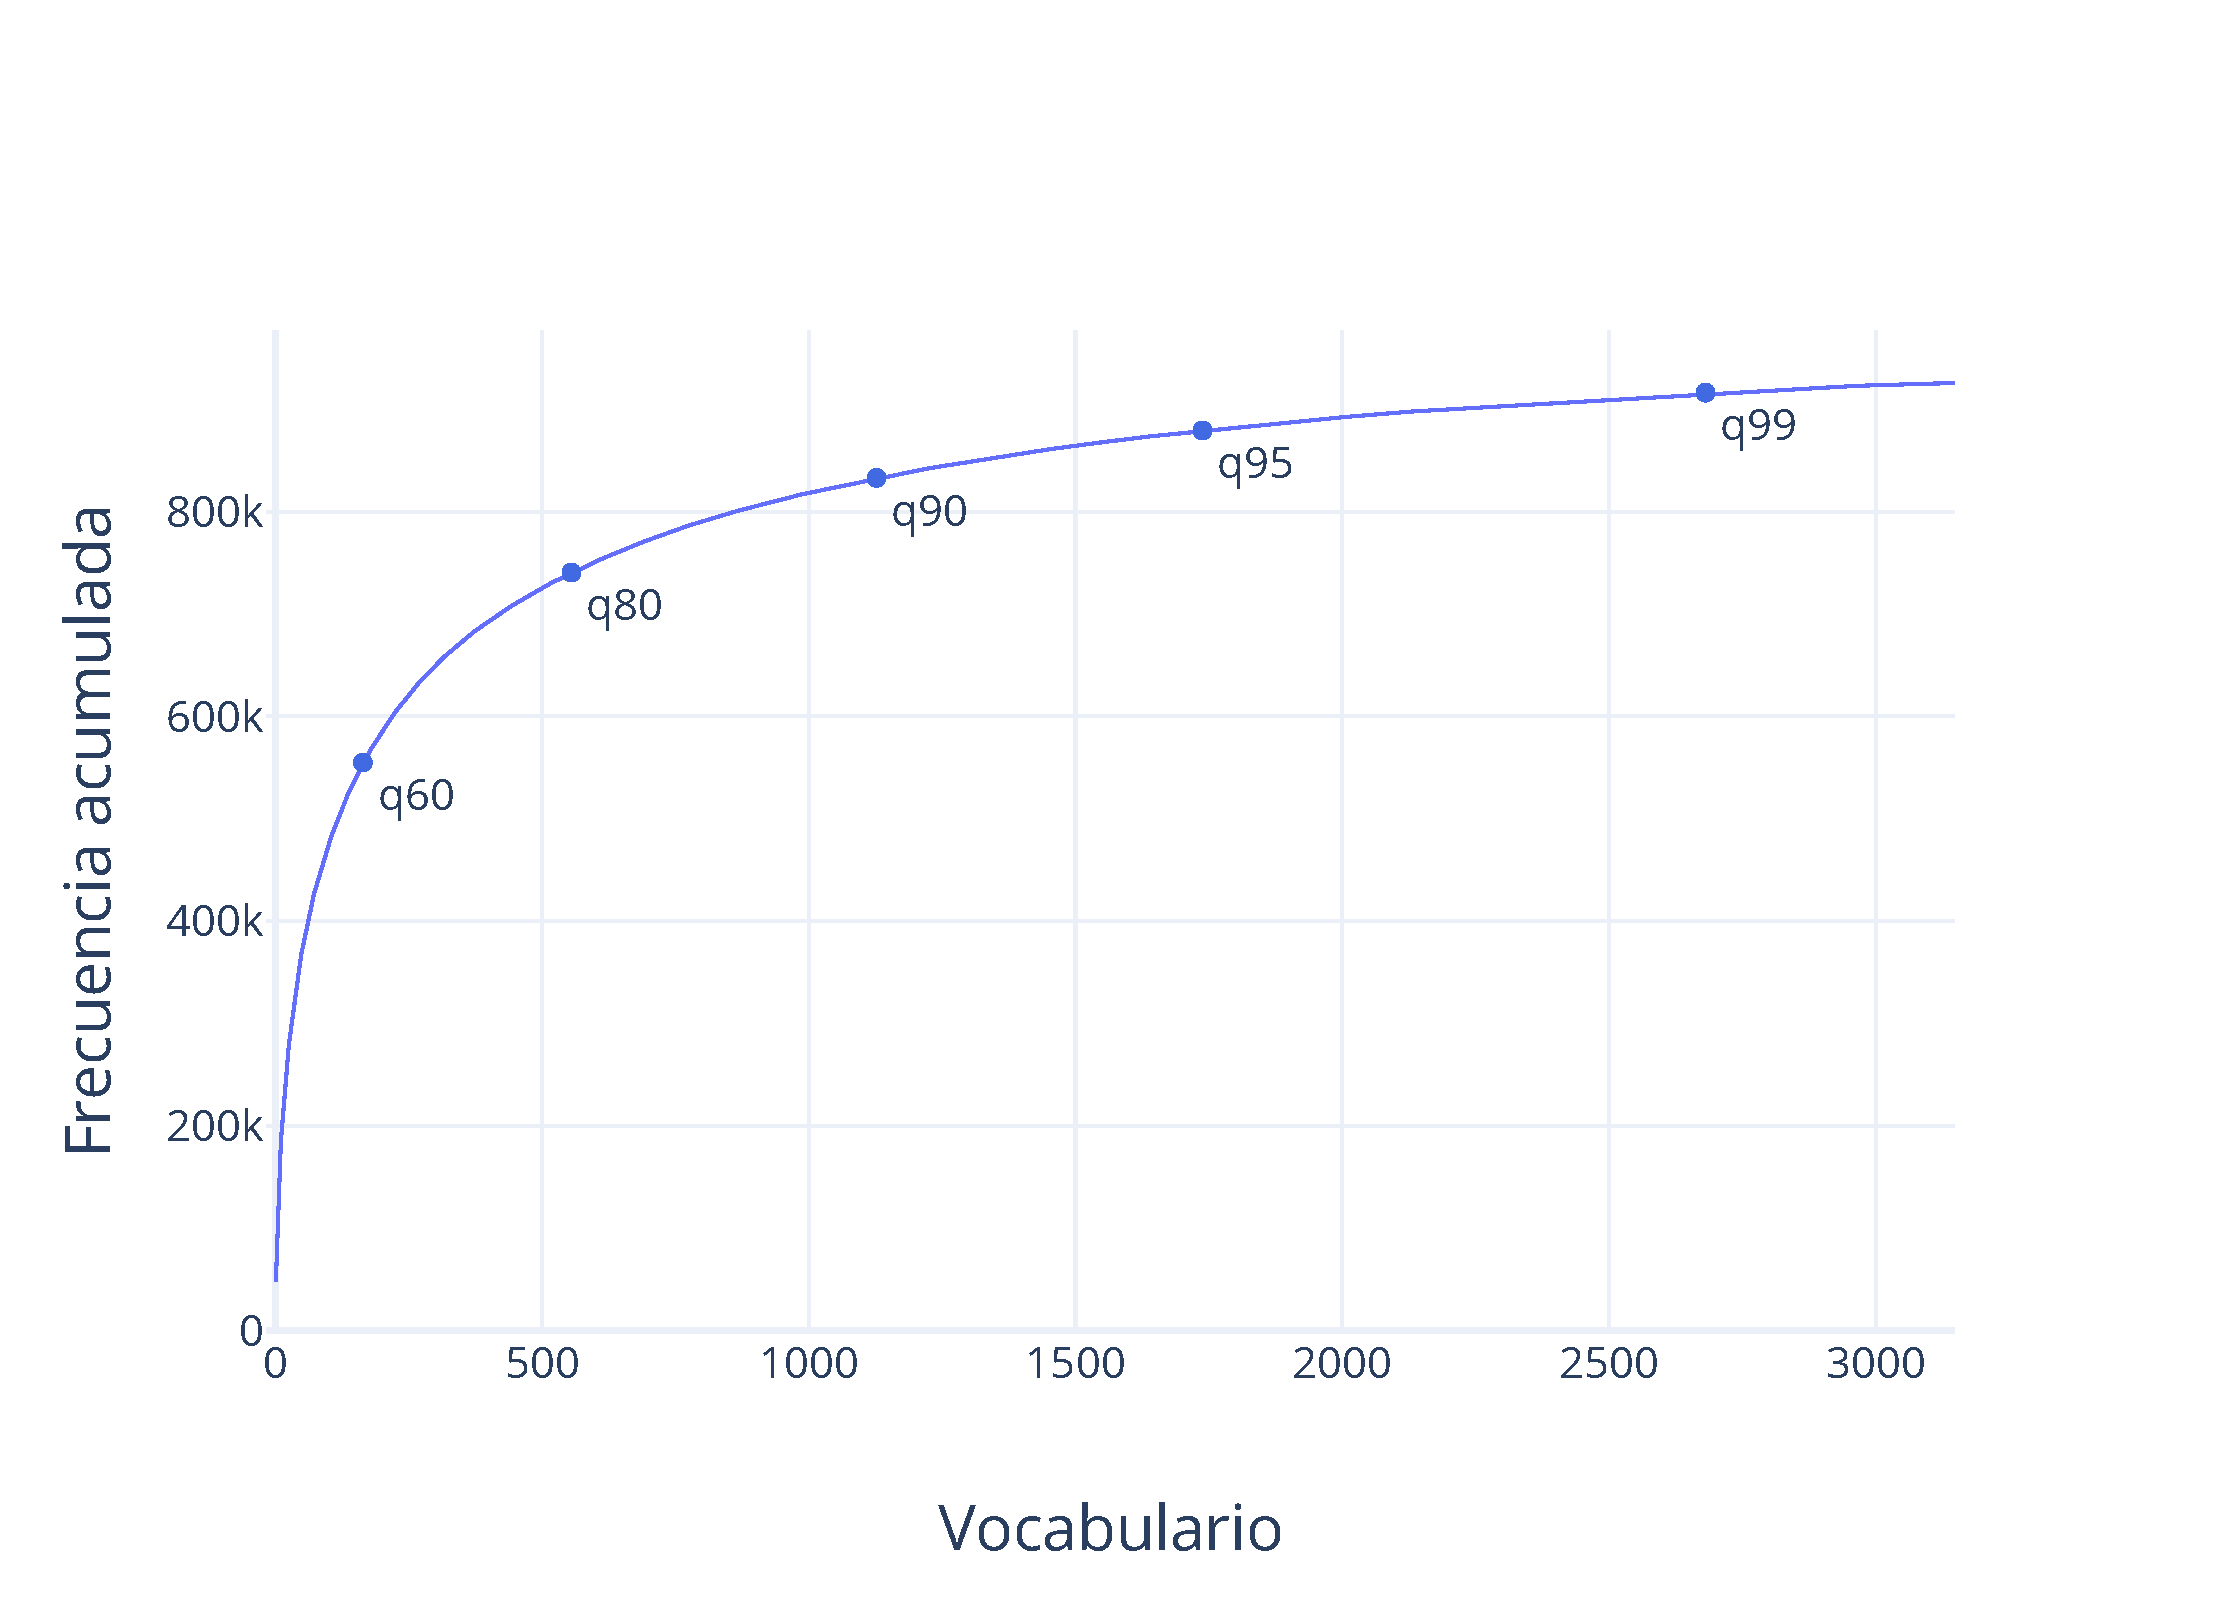
\includegraphics[trim={1.155cm 1.3cm 0 0},clip,width=0.6\textwidth]{ch4/cum_dist_3.eps}
    \caption{Frecuencia acumulada del vocabulario en orden decreciente de ocurrencia aplicando hasta el tercer nivel de procesamiento.}
    \label{img:cum_dist3}
\end{figure}

En cuarto lugar, se filtran palabras usando el vocabulario extraído del SUC. En la Figura \ref{img:cum_dist4} se observa que el vocabulario se redujo a 2,902 y el la cantidad de \textit{tokens} a 901,745. En este caso la variación no fue menos significativa, alrededor de un 8\% en el tamaño del vocabulario y de un 3\% en el caso de los \textit{tokens}.\\

\begin{figure}
    \centering
    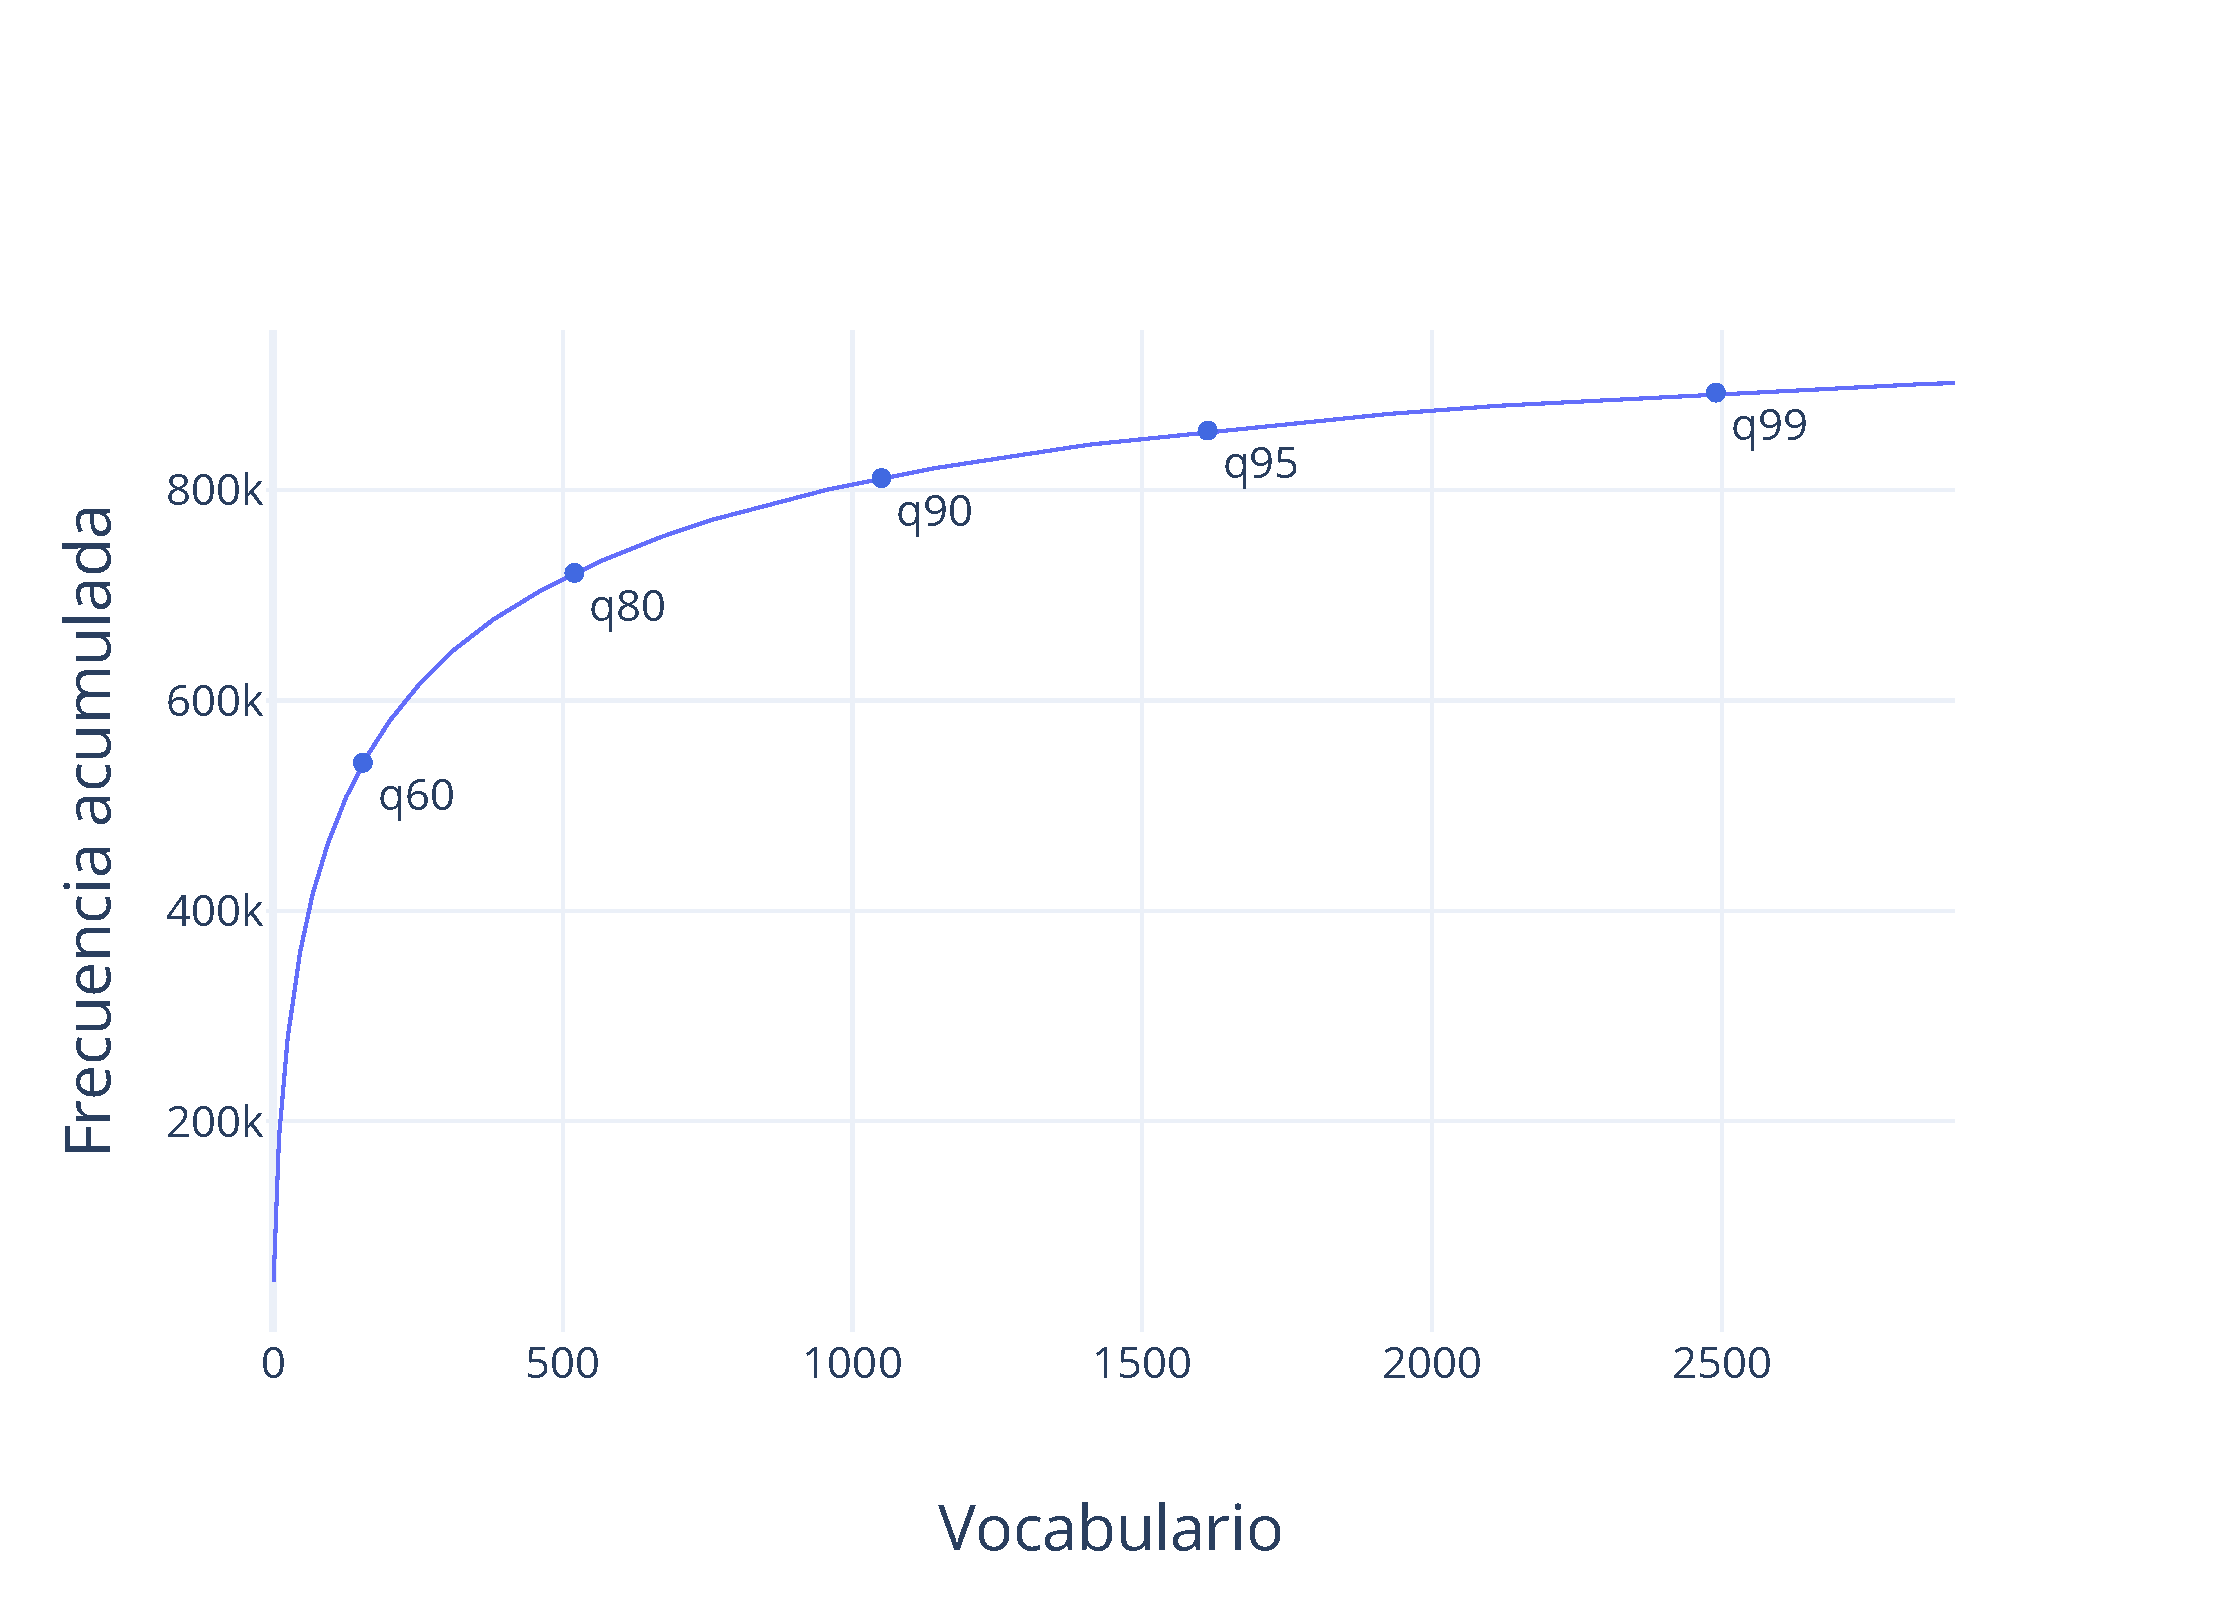
\includegraphics[trim={1.155cm 1.3cm 0 0},clip,width=0.6\textwidth]{ch4/cum_dist_4.eps}
    \caption{Frecuencia acumulada del vocabulario en orden decreciente de ocurrencia aplicando hasta el cuarto nivel de procesamiento.}
    \label{img:cum_dist4}
\end{figure}

En quinto lugar, se eliminan las \textit{stopwords}, de la Figura \ref{img:cum_dist5} se puede observar que significó una reducción significativa de tanto el vocabulario como del número de \textit{tokens}, respectivamente en 32\% (1,960 palabras) y 45\% (495,182 \textit{tokens}). La reducción abrupta en la cantidad de \textit{tokens} se debe principalmente a que las \textit{stopwords} son parte de las palabras más frecuentes dentro del corpus.\\

\begin{figure}
    \centering
    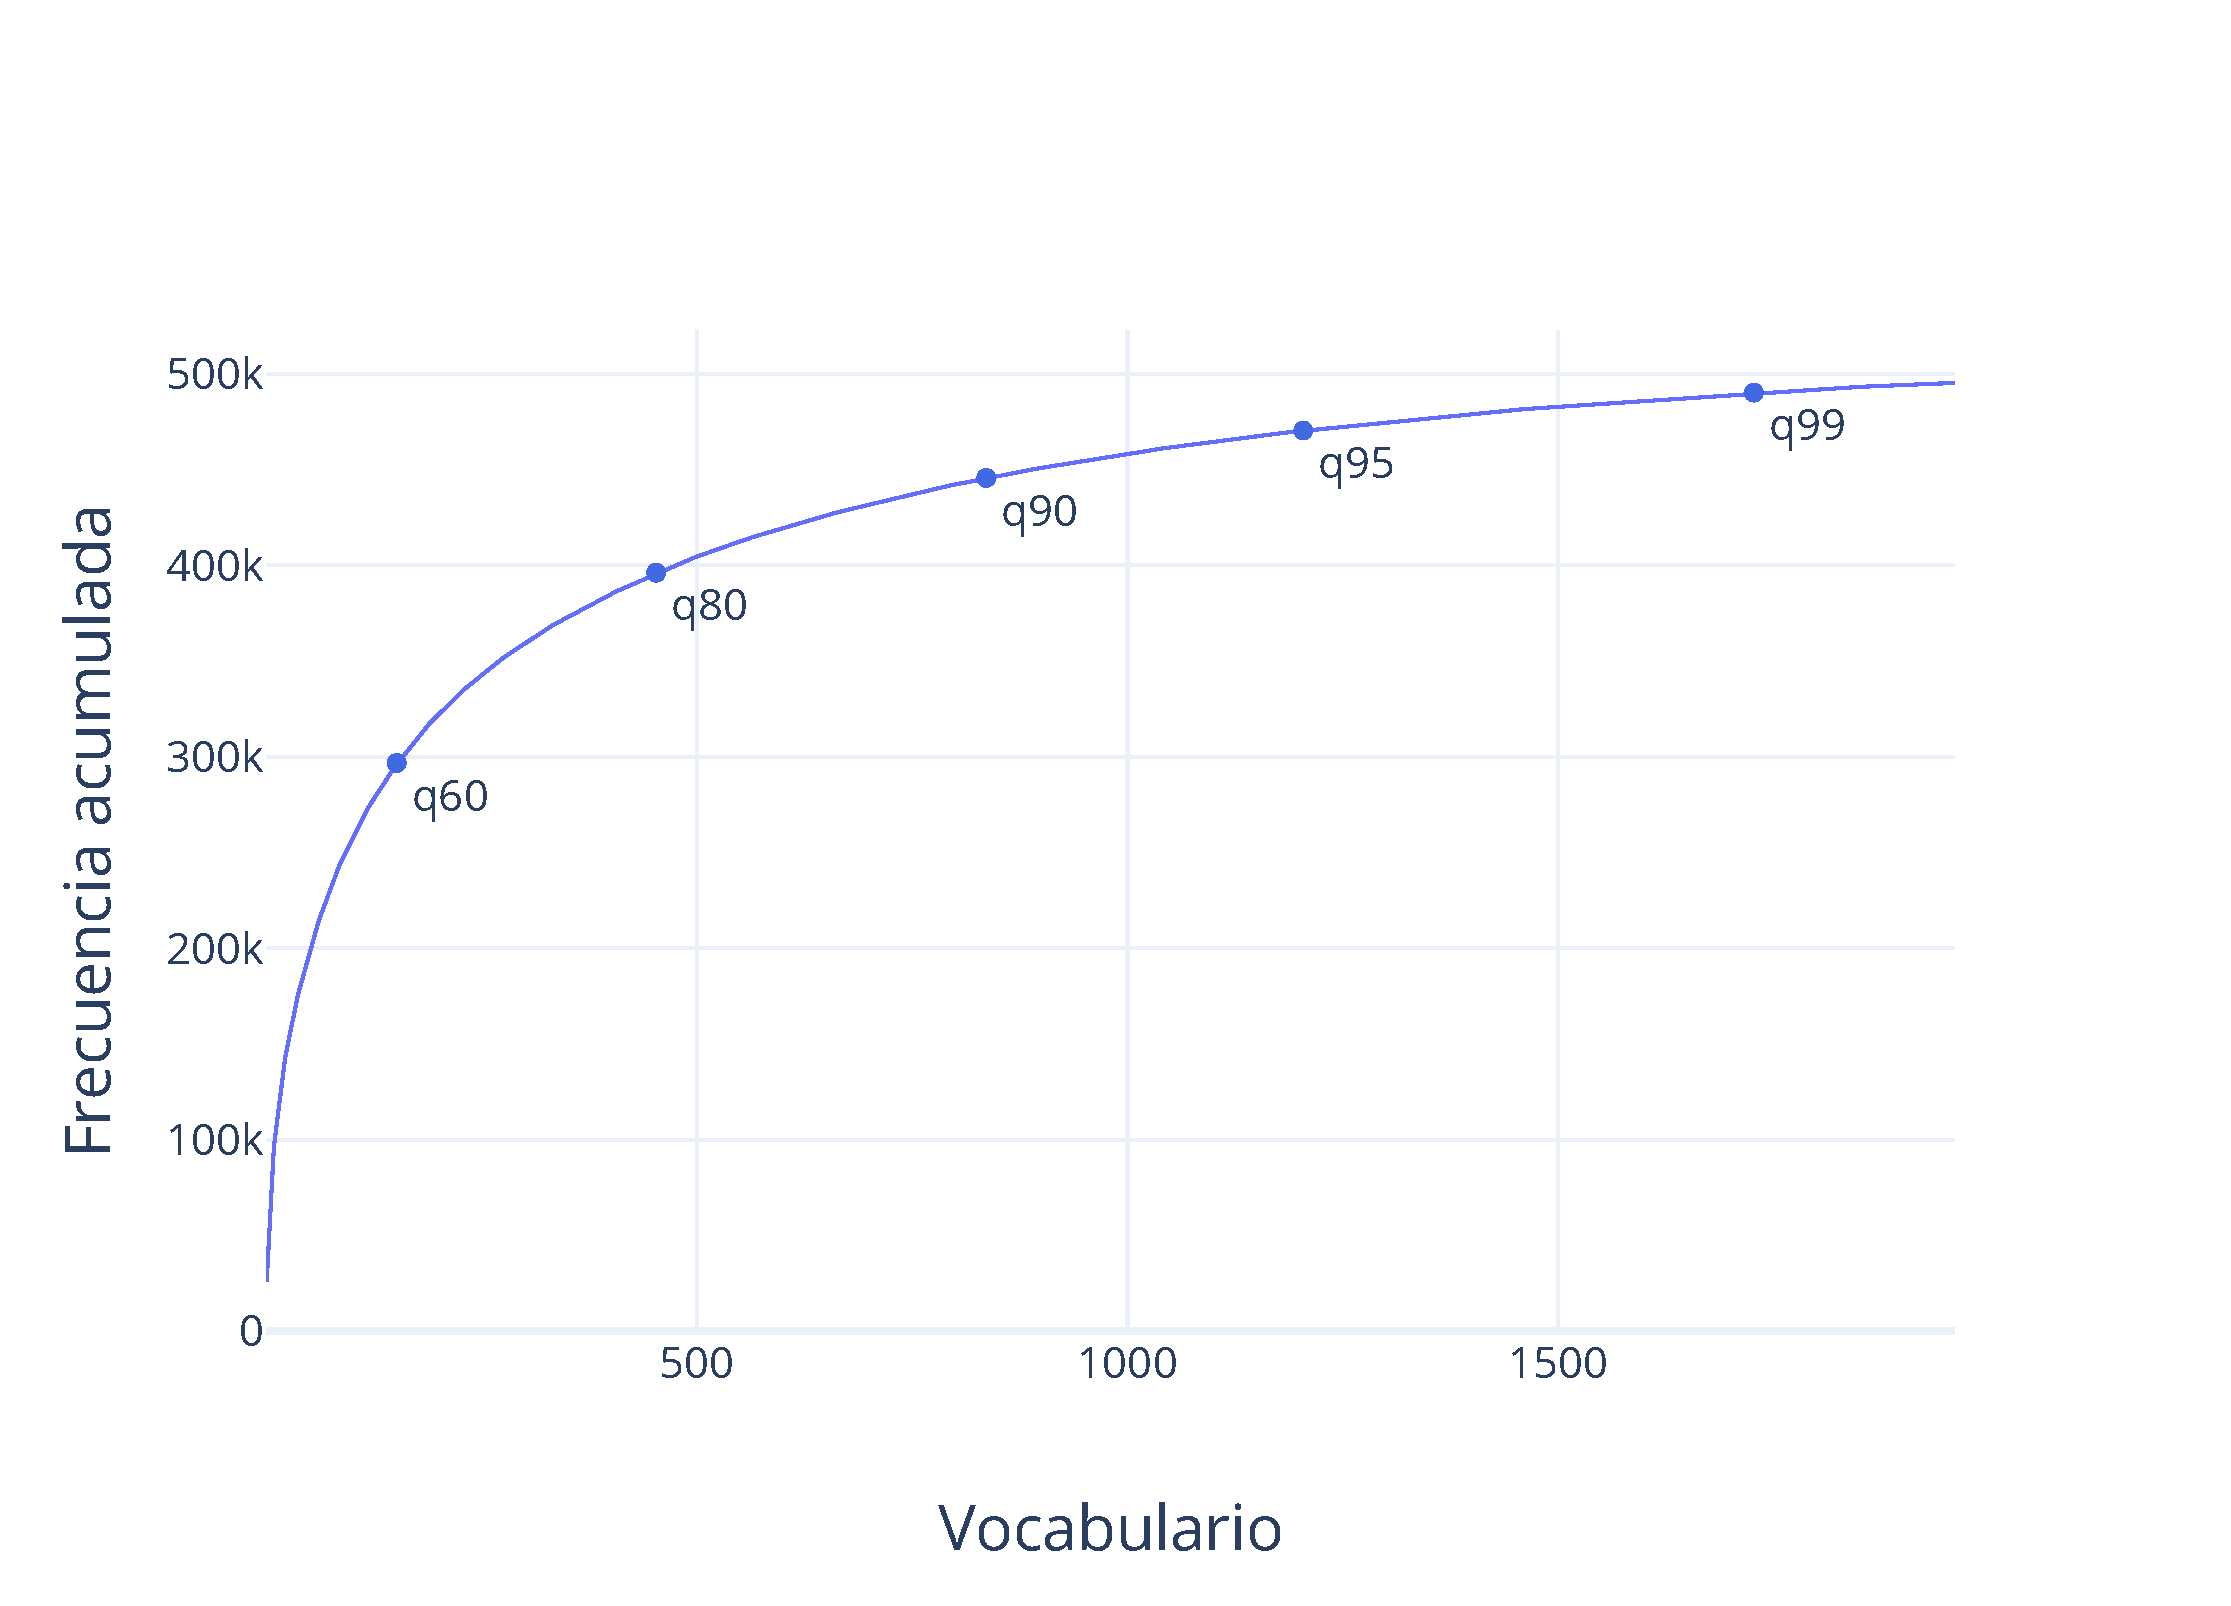
\includegraphics[trim={1.155cm 1.3cm 0 0},clip,width=0.6\textwidth]{ch4/cum_dist_5.eps}
    \caption{Frecuencia acumulada del vocabulario en orden decreciente de ocurrencia aplicando hasta el quinto nivel de procesamiento.}
    \label{img:cum_dist5}
\end{figure}

Por último, se eliminan los documentos con menos de 5 palabras, de la Figura \ref{img:cum_dist6} se puede observar que implicó una reducción de alrededor del 20\% en el tamaño del corpus y del 8\% en el número de \textit{tokens}.

\begin{figure}
    \centering
    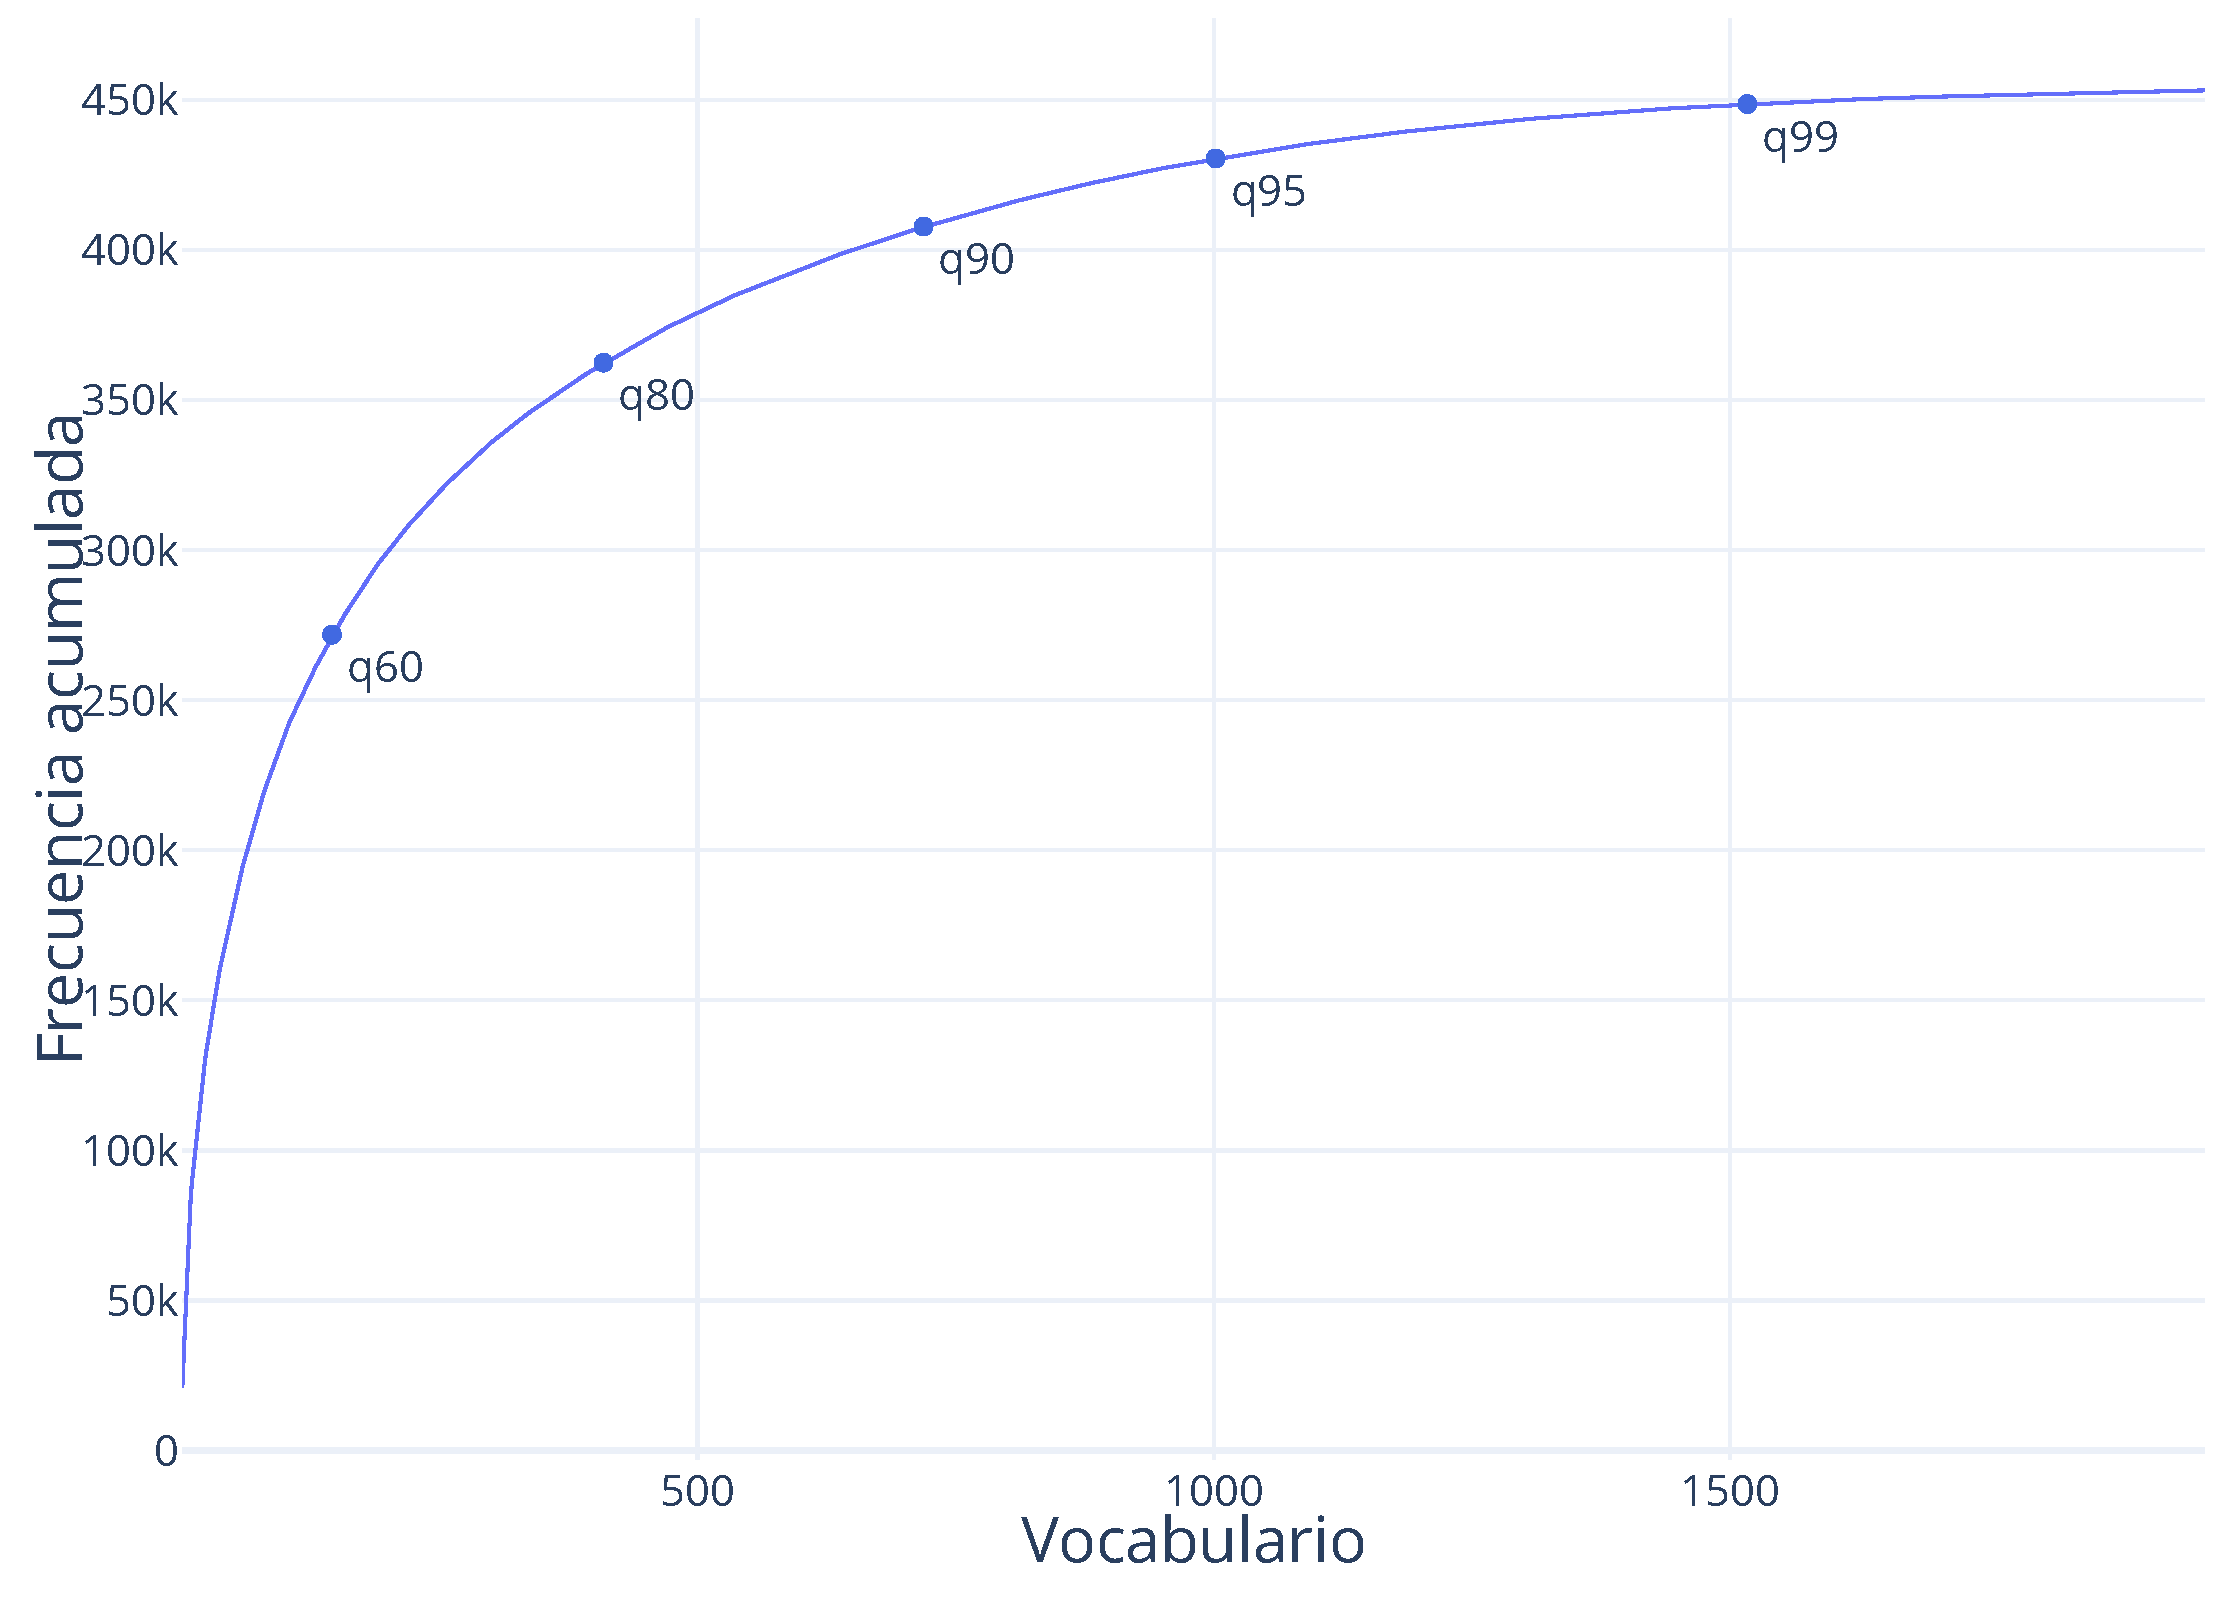
\includegraphics[trim={1.155cm 1.3cm 0 0},clip,width=0.6\textwidth]{ch4/cum_dist_6.eps}
    \caption{Frecuencia acumulada del vocabulario en orden decreciente de ocurrencia aplicando hasta el sexto nivel de procesamiento.}
    \label{img:cum_dist6}
\end{figure}

En la tabla \ref{table:processing_stats} se muestra un cuadro resumen con estadísticas del corpus bajo distintos niveles de procesamiento. De aquí se extrae que el tamaño del vocabulario, el corpus y la cantidad de \textit{tokens} se redujo en alrededor de un 98\%, un 20\% y un 76\% respectivamente.

\begin{table}[H]
    \begin{tabular}{|c|c|c|c|}
    \hline
    procesamiento & documentos & vocabulario & tokens  \\ \hline
    t             & 49,015      & 93,203       & 2,030,980 \\ \hline
    t+ch          & 49,003      & 42,921       & 1,028,412 \\ \hline
    t+ch+f        & 48,988      & 3,148        & 925,693  \\ \hline
    t+ch+f+v      & 48,988      & 2,902        & 901,745  \\ \hline
    t+ch+f+v+s    & 48,566      & 1,960        & 495,182  \\ \hline
    t+ch+f+v+s+d  & 38,850      & 1,960        & 453,206  \\ \hline
    \end{tabular}
    \caption{Estadísticas del corpus bajo distintos niveles de procesamientos, \textbf{t}: tokenización, \textbf{ch}: procesamiento de caracteres, \textbf{f}: filtro por frecuencia, \textbf{v}: filtro por vocabulario, \textbf{s}: eliminación de \textit{stopwords}, \textbf{d}: eliminación de documentos.}
    \label{table:processing_stats}
    \end{table}

En la tabla \ref{table:innovation_rate} se muestra el detalle del vocabulario para cada una de las épocas tras procesar el corpus, de aquí se extrae que en promedio un 12.83\% del vocabulario se olvida de una época a otra y un 18.92\% es nuevo, en otras palabras, en promedio alrededor de un 32\% del vocabulario no es común entre tópicos de épocas adyacentes. Esto justifica la necesidad de utilizar medidas de similitud robustas a cambios en el vocabulario, permitiendo así una comparación más justa entre tópicos sin vocabulario común.

\begin{table}[H]
    \begin{tabular}{|c|r|r|r|r|}
    \hline
    \textbf{época} & \multicolumn{1}{c|}{\textbf{t-1}} & \multicolumn{1}{c|}{\textbf{t}} & \multicolumn{1}{c|}{\textbf{t-1 {[}\%{]}}} & \multicolumn{1}{l|}{\textbf{t {[}\%{]}}} \\ \hline
    2              & 1,145                              & 1,187                            & 14.41                                      & 18.08                                    \\ \hline
    3              & 1,187                              & 1,281                            & 13.56                                      & 21.48                                    \\ \hline
    4              & 1,281                              & 1,329                            & 13.35                                      & 17.10                                    \\ \hline
    5              & 1,329                              & 1,405                            & 12.57                                      & 18.28                                    \\ \hline
    6              & 1,405                              & 1,537                            & 10.25                                      & 19.64                                    \\ \hline
    \end{tabular}
    \caption{Evolución del vocabulario en el tiempo, \textbf{t-1}: corresponde al vocabulario del período anterior a la época respectiva, \textbf{t}: corresponde al vocabulario de la época actual, \textbf{t-1[\%]}: porcentaje de palabras del período $t-1$ que ya no están en el período $t$ y \textbf{t[\%]}: porcentaje de palabras del período $t$ que no están en el período $t-1$.}
    \label{table:innovation_rate}.
\end{table}

\section{Análisis cuantitativo de resultados}
\label{sec:quantative}

En esta sección se describen los resultados cuantitativos de aplicar la metodología propuesta al corpus descrito en la sección \ref{sec:data}. En primer lugar, se analiza el comportamiento temporal de los tópicos bajo distintos puntos operantes $\zeta$ para podar el grafo \textit{fully-connected}. En segundo lugar, se analizan los resultados de aplicar la heurística descrita en \ref{sec:wmd_complexity}, la cual mejora los tiempos de construcción del grafo de similitud a costa de pérdida en precisión.

\subsection{Grafo de similitud temporal}

Como se menciona en la sección \ref{sec:build_graph}, el grafo temporal se construye relacionando los tópicos de épocas adyacentes a través de una medida de similitud, los tópicos son descubiertos usando el modelo HDP y WMD por medida de similitud. En base a un punto operante $\zeta \in [0,1]$ de la cdf de la similitud del grafo completo se determina el úmbral de corte. Aquellos arcos con similitud menor a este úmbral son eliminados. De esta forma la elección del úmbral no depende fuertemente de la medida de similitud escogida. En la Figura \ref{img:cdf_wmd} se ilustra la cdf del grafo \textit{fully-connected} obtenido de aplicar la metodología propuesta al corpus descrito en la sección \ref{sec:data}.

\begin{figure}
    \centering
    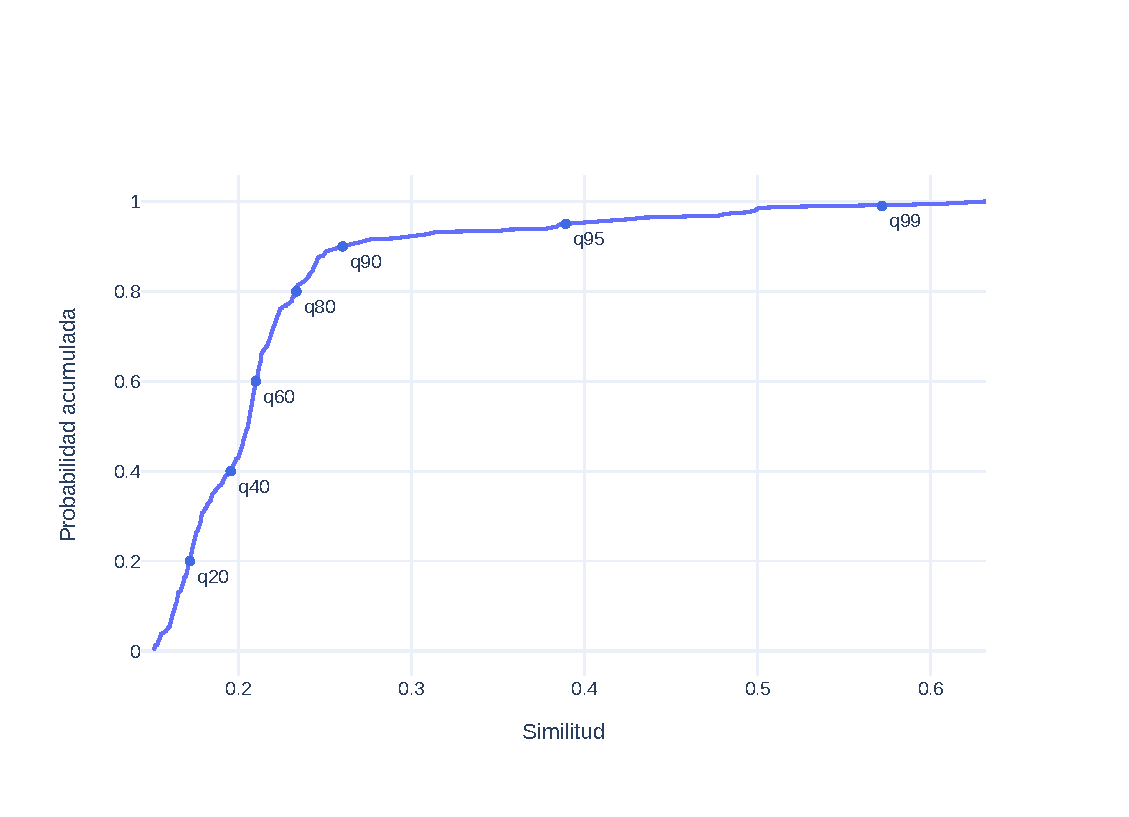
\includegraphics[width=\textwidth]{ch4/cdf.eps}
    \caption{Estimación empírica de la cdf de la similitud WMD entre tópicos del grafo \textit{fully-conected}.}
    \label{img:cdf_wmd}
\end{figure}

En la Figura \ref{img:temporal_similarity_graphs} se muestran los grafos resultantes tras aplicar distintos puntos operantes $\zeta$. Como es esperado, un incremento de $\zeta$ resulta en un incremento en la \textit{sparsity} del grafo temporal.

\begin{figure}
\centering
\subfloat[$\zeta$ = 0]{
  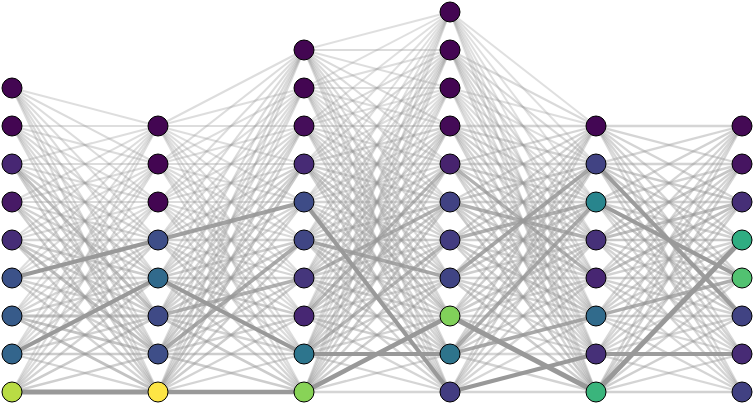
\includegraphics[width=0.4\textwidth]{ch4/graph_q100.png}
}
\subfloat[$\zeta$ = 0.9]{
  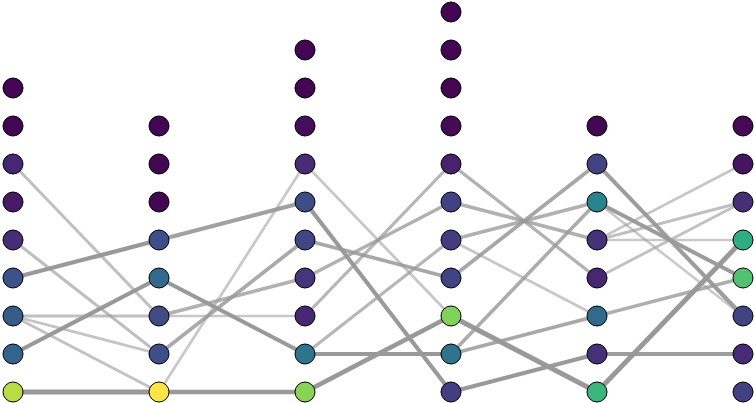
\includegraphics[width=0.4\textwidth]{ch4/graph_q100_e90.png}
}\\
\subfloat[$\zeta$ = 0.95]{
  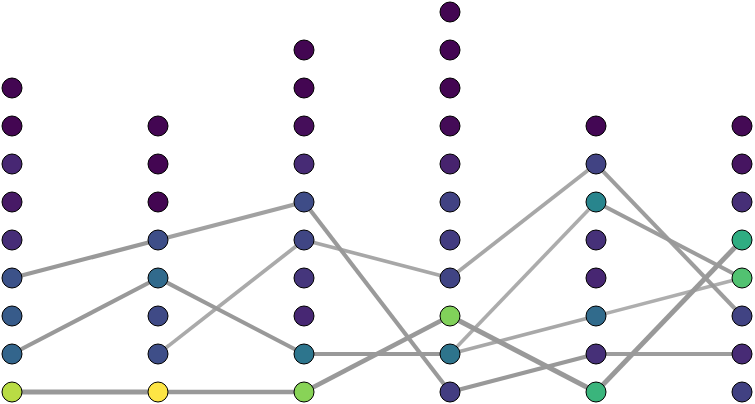
\includegraphics[width=0.4\textwidth]{ch4/graph_q100_e95.png}
}
\subfloat[$\zeta$ = 0.99]{
  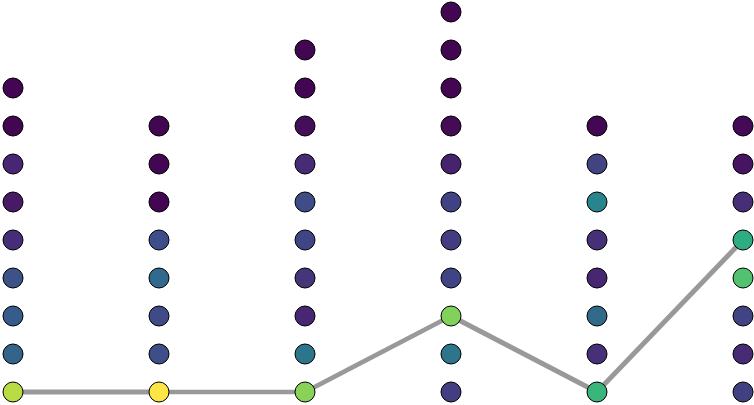
\includegraphics[width=0.4\textwidth]{ch4/graph_q100_e99.png}
}\\
\caption{Grafo de similitud temporal. Los grafos corresponden al mismo corpus y fueron construidos usando el mismo conjunto de tópicos con WMD como medida de similitud, pero bajo diferentes puntos operantes $\zeta$ de la CDF. El eje horizontal denota el tiempo en años, partiendo en el 2011 hasta el 2016, donde cada columna de tópicos corresponde a una época específica. Mientras más claro sea el color del nodo que representa un tópico más popularidad posee en su correspondiente época y mientras mayor es el grosor del arco entre dos tópicos mayor es su similitud.}
\label{img:temporal_similarity_graphs}
\end{figure}

En el grafo podado se pueden identificar diferentes dinamismos en cada época, como nacimiente, muerte, evolución, fusión y división. Un tópico nace en una época si en la época anterior no posee antecesores. La época de muerte de un tópico se identifica como aquella en que no tiene ningún descendiente. Un tópico evoluciona si posee un único antecesor. La fusión ocurre en una época cuando un tópico tiene más de un antecesor. En cambio, la división ocurre cuando hay dos o más tópicos de una época que comparten un antecesor.\\

En la Figura \ref{img:topics_evolution} se muestra la proporción de tópicos que nacen, mueren, fusionan, y dividen por época, normalizando por el número total de tópicos inferido en esa época. Se puede observar que al incrementar $\zeta$ la proporción de tópicos que nacen y mueren aumenta significativamente, puesto que al ser mayor el úmbral de corte menos ascendentes y descendientes se tienen, por otro lado, la división y fusión decrecen, debido a la menor presencia de conexiones.

\begin{figure}
    \centering
    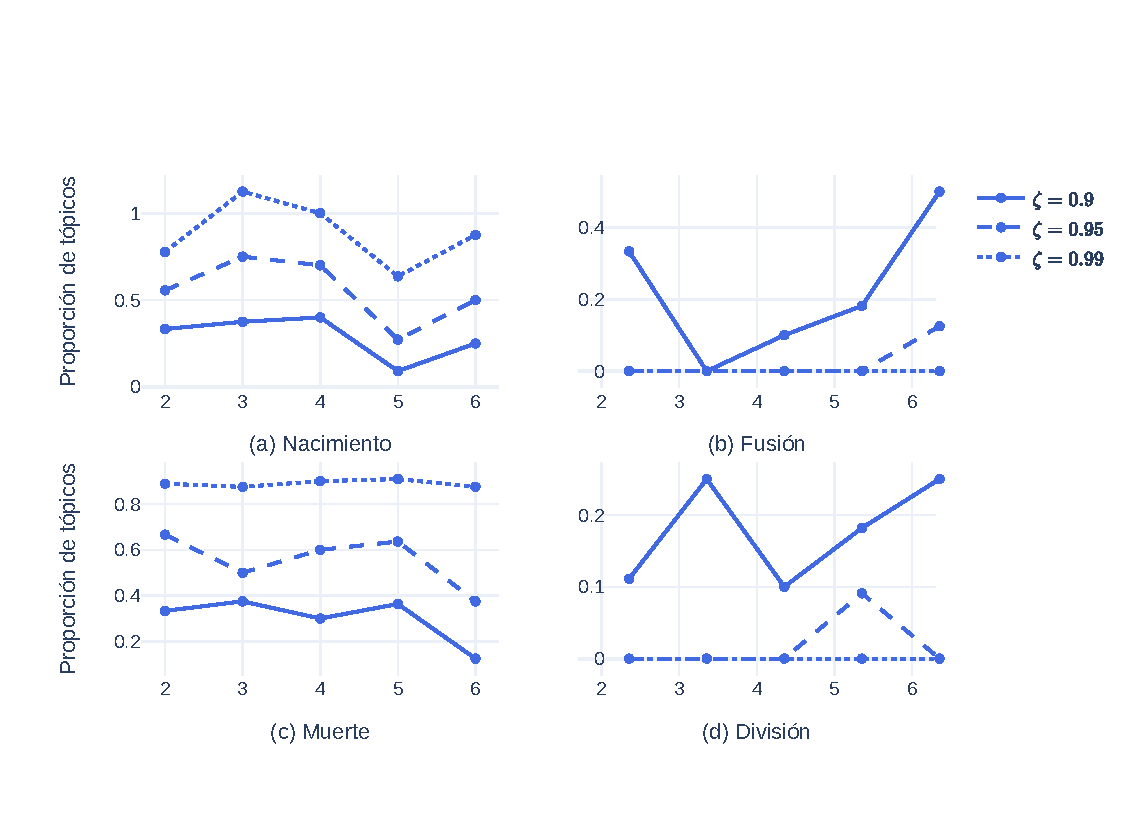
\includegraphics[width=\textwidth]{ch4/topics_evolution.eps}
    \caption{Proporción de tópicos que nacen, mueren, fusionan y dividen por época, normalizando por el número total de tópicos inferido en esa época, bajo diferentes puntos operantes $\zeta$.}
    \label{img:topics_evolution}
\end{figure}

\subsection{Heurística de mejora del tiempo de construcción del grafo de similitud}

WMD es una medida intensiva en recursos computacionales, por lo que se requiere de heurísticas para escalar la metodología a un gran volumen de datos. Como se menciona en la sección \ref{sec:wmd_complexity} una forma de reducir significativamente el tiempo de creación del grafo temporal es utilzar el top N de palabras más probables del tópico que expliquen determinado porcentaje de la distribución acumulada. A la hora de aplicar esta heurística se debe tener en cuenta la posible pérdida de información al representar un tópico con un vocabulario reducido. Sea $G_{\zeta}$ el grafo obtenido al aplicar tras podar el grafo completo con un punto operante $\zeta$ y $G^{'}_{\zeta}$ el grafo aproximado de aplicar la heurística, con $E$ y $E^{'}$ los conjuntos de arcos respectivos. Luego, el porcentaje de arcos correctos de la heurística corresponde a la cardinalidad de la intersección divida por la cardinalidad de la unión, matemáticamente:

\begin{equation}
  \frac{|E\cap E^{'}|}{|E\cup E^{'}|}
\end{equation}

En la Figura \ref{img:speedup} se muestra la mejora en \textit{speedup} y el incremento en error al usar un porcentaje menor de la cdf del tópico para construir el grafo de similitud temporal. Utilizando el 20\% de la cdf la construcción del grafo de similitud disminuye en más de 1,207 veces, esto bajo un error medianamente aceptable del orden del 10-30\%. Si se utiliza un 60\% de la cdf el tiempo mejora en casi 137 veces, siendo el error menor al 10\%. Por otro lado, si se utiliza un 90\% de la cdf el error es inferior al 5\%, siendo el speedup es aproximadamente 8 veces superior a utilizar el vocabulario completo del tópico en la construcción del grafo temporal.

\begin{figure}
    \centering
    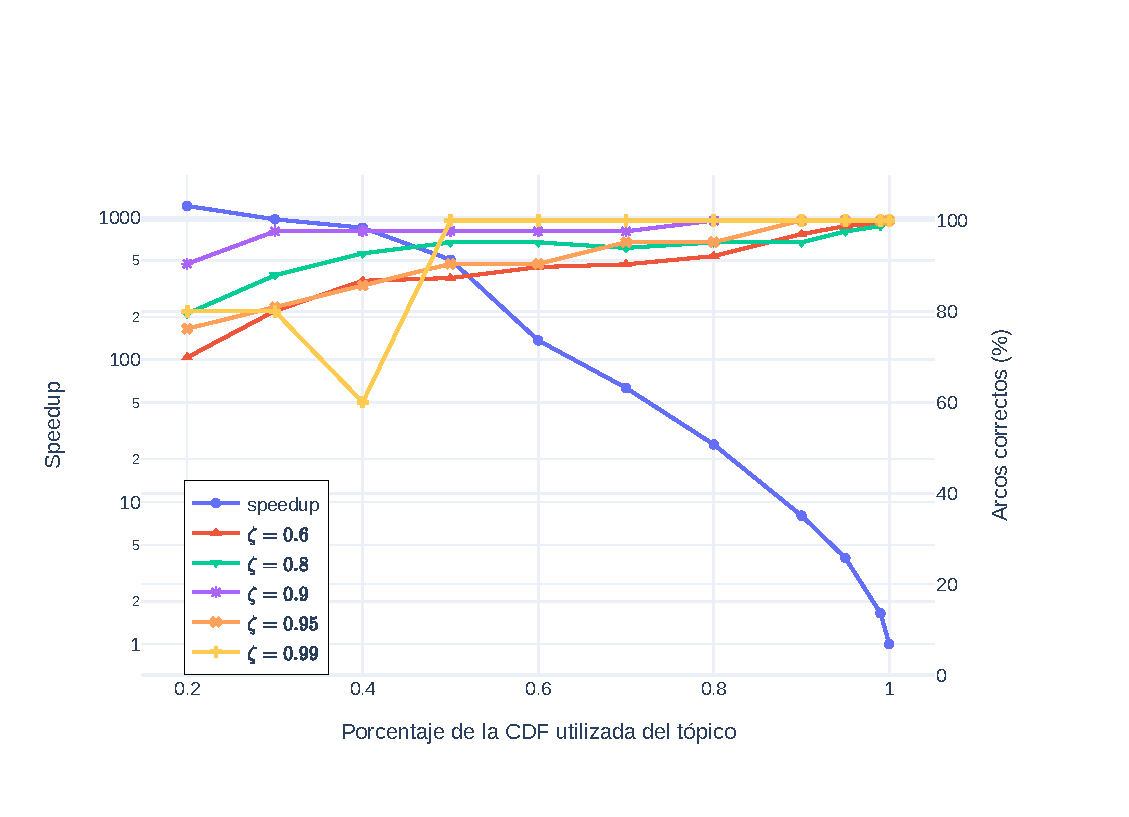
\includegraphics[width=\textwidth]{ch4/speedup.eps}
    \caption{\textit{Speedup} y porcentaje de arcos correctos al utilizar un menor porcentaje de la cdf de los tópicos en la construcción del grafo de similitud. El error de la heurística es mostrado para diferentes puntos operantes $\zeta$ utilizados para podar el grafo completo.} 
    \label{img:speedup}
\end{figure}

\section{Análisis cualitativo de resultados}
\label{sec:qualitative}

En esta sección se realiza un análisis cualitativo de los tópicos descubiertos y su evolución. El análisis es realizado sobre el grafo podado con un punto operante $\zeta = 0.95$ mostrado en la Figura \ref{img:temporal_similarity_graphs}. En las siguientes dos subsecciones se analizan los dos tópicos más predominantes en el tiempo: en la sección \ref{sec:noviolence_topic} se estudia el robo no presencial y en la sección \ref{sec:violence_topic} se analiza el robo con violencia.

\subsection{Evolución del robo no presencial}
\label{sec:noviolence_topic}

En la Figura \ref{img:noviolence_topic} se muestra la evolución de uno de los tópicos más predominantes del grafo temporal. A diferencia de otros tópicos este tópico no presenta en el tiempo división, fusión ni desaparición. En base a las top 10 palabras más probables el tópico se puede caracterizar como un robo bajo las siguientes circunstancias: vehículo estacionado en la calle, sin la presencia del conductor, el conductor al regresar al lugar se percata de la ausencia del vehículo. Un nombre adecuado para este tópico podría ser \quotes{robo no presencial}, ya que se caracteriza por no contar con la presencia del conductor cuando ocurre el robo. Este tópico se caracteriza por su gran estabilidad en el tiempo, ya que en el top 10 se encuentran practicamente las mismas palabras. Por último, se observa una tendencia a la baja de la participación del tópico, en el año 2011 alrededor del 44\% de los \textit{tokens} provienen de este tópico y en el año 2016 se tiene un 32\%.

\def\topic[#1,#2,#3,#4,#5,#6]#7{
        \node[fill=#1, rounded corners, minimum height=#2, minimum width=#3, text width=4em] (#5) at #6 {}; 
        \node[anchor=#4,inner sep=2pt,] at (#5.#4)  {#7};
}
\def\tedge[#1,#2,#3,#4,#5];{ 
  \definecolor{color0}{RGB}{153,153,153}
  \draw[color=color0,#4,fill=white, line width=4*#5pt] (#1) -- #3
  (#2);  
}

\definecolor{color1}{RGB}{184,222,41}
\definecolor{color2}{RGB}{253,231,37}
\definecolor{color3}{RGB}{134,213,73}
\definecolor{color4}{RGB}{127,211,78}
\definecolor{color5}{RGB}{52,182,121}
\definecolor{color6}{RGB}{40,174,128}

\begin{figure}
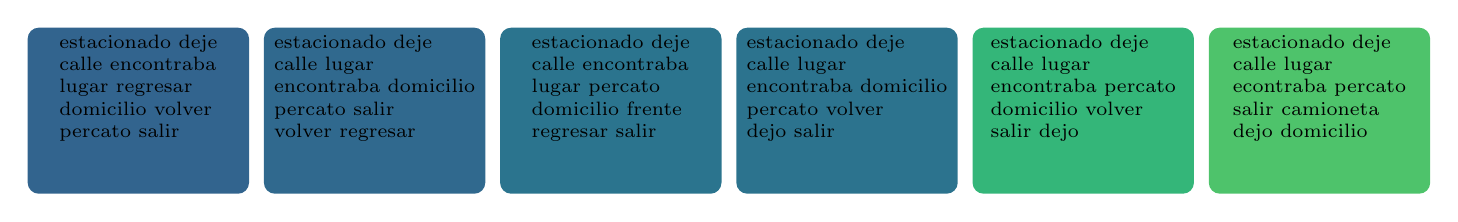
\begin{tikzpicture}
  \topic[color1,60,80,north,t1,(0,0)] {
     \scriptsize
     \begin{tabular}{l}
       estacionado deje\\
       calle encontraba\\
       lugar regresar\\
       domicilio volver\\
       percato salir
     \end{tabular}
  }
  \topic[color2,60,80,north,t2,(3,0)] {
     \scriptsize
     \begin{tabular}{l}
       estacionado deje\\
       calle lugar\\
       encontraba domicilio\\
       percato salir\\
       volver regresar
     \end{tabular}
  };
  \topic[color3,60,80,north,t3,(6,0)] {
     \scriptsize
     \begin{tabular}{l}
       estacionado deje\\
       calle encontraba\\
       lugar percato\\
       domicilio frente\\
       regresar salir
     \end{tabular}
  };
  \topic[color4,60,80,north,t4,(9,0)] {
     \scriptsize
     \begin{tabular}{l}
       estacionado deje\\
       calle lugar\\
       encontraba domicilio\\
       percato volver\\
       dejo salir
     \end{tabular}
  };
  \topic[color5,60,80,north,t5,(12,0)] {
     \scriptsize
     \begin{tabular}{l}
       estacionado deje\\
       calle lugar\\
       encontraba percato\\
       domicilio volver\\
       salir dejo
     \end{tabular}
  };
  \topic[color6,60,80,north,t6,(15,0)] {
     \scriptsize
     \begin{tabular}{l}
       estacionado deje\\
       calle lugar\\
       econtraba percato\\
       salir camioneta\\
       dejo domicilio
     \end{tabular}
  };
  \tedge[t1,t2,,,0.625];
  \tedge[t2,t3,,,0.586];
  \tedge[t3,t4,,,0.581];
  \tedge[t4,t5,,,0.632];
  \tedge[t5,t6,,,0.609];
\end{tikzpicture}
\caption{Evolución del tópico de robo de vehículo no presecial. El eje horizontal denota el tiempo en años, partiendo en el 2011 hasta el 2016. Mientras más claro el color del tópico más popularidad posee en su correspondiente época y mientras mayor es el grosor del arco entre dos tópicos mayor es su similitud.}
\label{img:noviolence_topic}
\end{figure}

\subsection{Evolución del robo con violenca}
\label{sec:violence_topic}

En la Figura \ref{img:violence_topic} se describe un tipo de robo de vehículo que se puede clasificar como robo con violencia. Este delito, se presenta de la siguiente forma: un conjunto de personas se bajan de un vehículo, intimidan al conductor mediante una pistola u otra arma de fuego, le quitan las llaves del vehículo y finalmente se llevan el vehículo dándose a la fuga. La participación de este tipo de robo se ha visto al alza, en el 2011 su participación era del 12\% y en el 2016 del 36\%, por lo que se ha convertido en un delito más a la moda, quitandole terreno al robo no presencial. A diferencia del tópico robo no presencial este presenta una fusión y división en el 2015. En ese año emerge del robo con violencia un subtópico popularmente conocido como \quotes{portonazo}, un robo con violencia que se caracteriza por la sustracción del vehículo en el portón de la casa de la víctima. Ese año coincide con la popularización de aquel \textit{modus operandi}. Al siguiente año el subtópico se vuelve a fusionar para formar parte del tópico robo con violencia de períodos anteriores.

\definecolor{color1}{RGB}{50,100,142}
\definecolor{color2}{RGB}{48,105,142}
\definecolor{color3}{RGB}{43,116,142}
\definecolor{color4}{RGB}{44,115,142}
\definecolor{color51}{RGB}{37,133,142}
\definecolor{color52}{RGB}{48,106,142}
\definecolor{color6}{RGB}{78,195,107}

\begin{figure}
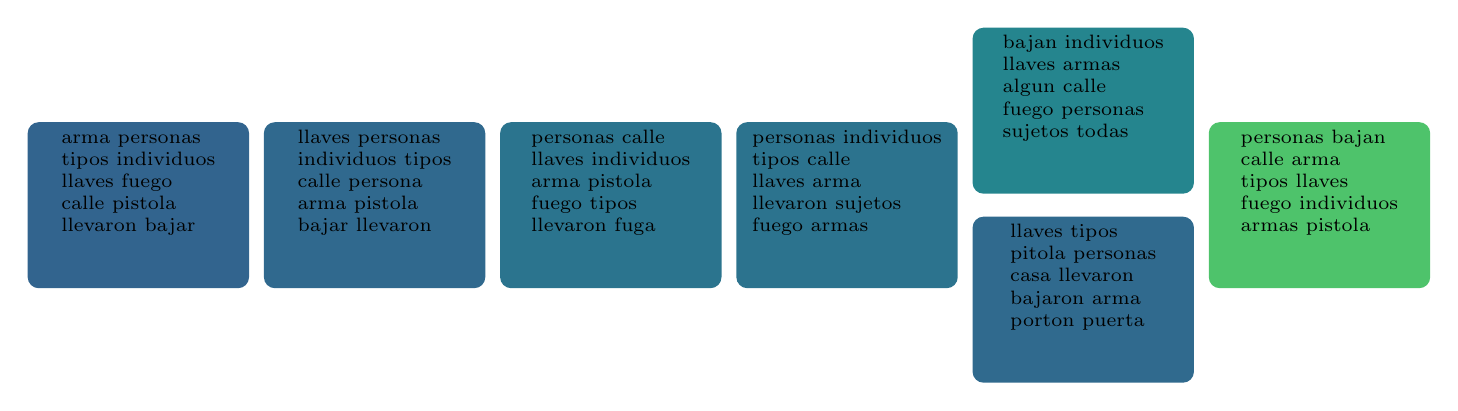
\begin{tikzpicture}
  \topic[color1,60,80,north,t1,(0,0)] {
     \scriptsize
     \begin{tabular}{l}
       arma personas\\
       tipos individuos\\
       llaves fuego\\
       calle pistola\\
       llevaron bajar
     \end{tabular}
  }
  \topic[color2,60,80,north,t2,(3,0)] {
     \scriptsize
     \begin{tabular}{l}
       llaves personas\\
       individuos tipos\\
       calle persona\\
       arma pistola\\
       bajar llevaron
     \end{tabular}
  };
  \topic[color3,60,80,north,t3,(6,0)] {
     \scriptsize
     \begin{tabular}{l}
       personas calle\\
       llaves individuos\\
       arma pistola\\
       fuego tipos\\
       llevaron fuga
     \end{tabular}
  };
  \topic[color4,60,80,north,t4,(9,0)] {
     \scriptsize
     \begin{tabular}{l}
       personas individuos\\
       tipos calle\\
       llaves arma\\
       llevaron sujetos\\
       fuego armas
     \end{tabular}
  };
  \topic[color51,60,80,north,t51,(12,1.2)] {
     \scriptsize
     \begin{tabular}{l}
       bajan individuos\\
       llaves armas\\
       algun calle\\
       fuego personas\\
       sujetos todas
     \end{tabular}
  };
  \topic[color52,60,80,north,t52,(12,-1.2)] {
     \scriptsize
     \begin{tabular}{l}
       llaves tipos\\
       pitola personas\\
       casa llevaron\\
       bajaron arma\\
       porton puerta
     \end{tabular}
  };
  \topic[color6,60,80,north,t6,(15,0)] {
     \scriptsize
     \begin{tabular}{l}
       personas bajan\\
       calle arma\\
       tipos llaves\\
       fuego individuos\\
       armas pistola
     \end{tabular}
  };
  \tedge[t1,t2,,,0.499];
  \tedge[t2,t3,,,0.498];
  \tedge[t3,t4,,,0.5];
  \tedge[t4,t51,,,0.422];
  \tedge[t4,t52,,,0.405];
  \tedge[t51,t6,,,0.395];
  \tedge[t52,t6,,,0.483];
\end{tikzpicture}
\caption{Evolución del tópico de robo con violencia de vehículo. El eje horizontal denota el tiempo en años, partiendo en el 2011 hasta el 2016. Mientras más claro el color del tópico más popularidad posee en su correspondiente época y mientras mayor es el grosor del arco entre dos tópicos mayor es su similitud.}
\label{img:violence_topic}
\end{figure}
